% !TeX spellcheck = en-US
% !TeX encoding = utf8
% !TeX program = lualatex
% !BIB program = biber
% -*- coding:utf-8 mod:LaTeX -*-


% vv  scroll down to line 200 for content  vv


\let\ifdeutsch\iffalse
\let\ifenglisch\iftrue
\input{pre-documentclass}
\documentclass[
  % fontsize=11pt is the standard
  a4paper,  % Standard format - only KOMAScript uses paper=a4 - https://tex.stackexchange.com/a/61044/9075
  twoside,  % we are optimizing for both screen and two-side printing. So the page numbers will jump, but the content is configured to stay in the middle (by using the geometry package)
  bibliography=totoc,
  %               idxtotoc,   %Index ins Inhaltsverzeichnis
  %               liststotoc, %List of X ins Inhaltsverzeichnis, mit liststotocnumbered werden die Abbildungsverzeichnisse nummeriert
  headsepline,
  cleardoublepage=empty,
  parskip=half,
  %               draft    % um zu sehen, wo noch nachgebessert werden muss - wichtig, da Bindungskorrektur mit drin
  draft=false
]{scrbook}
\input{config}


\usepackage[
  title={Transformed Sparse Grids for high-dimensional models},
  author={Christopher Schnick},
  type=master,
  institute=ipvs, % or other institute names - or just a plain string using {Demo\\Demo...}
  course={Informatik},
  examiner={Prof.\ Dr.\ Dirk Pflüger},
  supervisor={Dr. Michael Rehme},
  startdate={April 24, 2021},
  enddate={October 24, 2021}
]{scientific-thesis-cover}

\makeindex


\newtheorem{proof}{Proof}
\newtheorem{lemma}{Lemma}
\newtheorem{theorem}{Theorem}
\DeclareMathOperator*{\argmin}{arg\,min}
\DeclareMathOperator*{\argmax}{arg\,max}

\begin{document}

%tex4ht-Konvertierung verschönern
\iftex4ht
  % tell tex4ht to create picures also for formulas starting with '$'
  % WARNING: a tex4ht run now takes forever!
  \Configure{$}{\PicMath}{\EndPicMath}{}
  %$ % <- syntax highlighting fix for emacs
  \Css{body {text-align:justify;}}

  %conversion of .pdf to .png
  \Configure{graphics*}
  {pdf}
  {\Needs{"convert \csname Gin@base\endcsname.pdf
      \csname Gin@base\endcsname.png"}%
    \Picture[pict]{\csname Gin@base\endcsname.png}%
  }
\fi

%\VerbatimFootnotes %verbatim text in Fußnoten erlauben. Geht normalerweise nicht.

% DE: wird fuer Tabellen benötigt (z.B. >{centering\RBS}p{2.5cm} erzeugt einen zentrierten 2,5cm breiten Absatz in einer Tabelle
\newcommand{\RBS}{\let\\=\tabularnewline}

% EN: To avoid issues with Springer's \mathplus
%     See also http://tex.stackexchange.com/q/212644/9075
\providecommand\mathplus{+}

% EN: from hmks makros.tex - \indexify
\newcommand{\toindex}[1]{\index{#1}#1}

% DE: Anstatt $|x|$ $\abs{x}$ verwenden.
%     Die Betragsstriche skalieren automatisch, falls "x" etwas größer sein sollte...
\newcommand{\abs}[1]{\left\lvert#1\right\rvert}

% EN: For the algorithmic package
\newcommand{\commentchar}{\ensuremath{/\mkern-4mu/}}
\algrenewcommand{\algorithmiccomment}[1]{\hfill $\commentchar$ #1}

% DE: Seitengrößen - Gegen Schusterjungen und Hurenkinder...
\newcommand{\largepage}{\enlargethispage{\baselineskip}}
\newcommand{\shortpage}{\enlargethispage{-\baselineskip}}

\newcommand{\Hsquare}{%
  \text{\fboxsep=-.2pt\fbox{\rule{0pt}{1.4ex}\rule{1.4ex}{0pt}}}%
}
\newcommand\red{red\,{\setlength\fboxsep{0pt}\colorbox{persian_red}{\Hsquare}}\,\,}
\newcommand\reddot{red\,{\setlength\fboxsep{0pt}\colorbox{persian_red}{\Hsquare}}.}

\newcommand\green{green\,{\setlength\fboxsep{0pt}\colorbox{persian_green}{\Hsquare}}\,\,}
\newcommand\greendot{green\,{\setlength\fboxsep{0pt}\colorbox{persian_green}{\Hsquare}}.}
\newcommand\greencomma{green\,{\setlength\fboxsep{0pt}\colorbox{persian_green}{\Hsquare}},}

\newcommand\grey{grey\,{\setlength\fboxsep{0pt}\colorbox{silver}{\Hsquare}}\,\,}
\newcommand\greydot{grey\,{\setlength\fboxsep{0pt}\colorbox{silver}{\Hsquare}}.}

\newcommand\beige{beige\,{\setlength\fboxsep{0pt}\colorbox{eggshell}{\Hsquare}}\,\,}
\newcommand\beigedot{beige\,{\setlength\fboxsep{0pt}\colorbox{eggshell}{\Hsquare}}.}

\newcommand\lightblue{light blue\,{\setlength\fboxsep{0pt}\colorbox{light_cornflower_blue}{\Hsquare}}\,\,}
\newcommand\lightbluedot{light blue\,{\setlength\fboxsep{0pt}\colorbox{light_cornflower_blue}{\Hsquare}}.}

\newcommand\darkblue{dark blue\,{\setlength\fboxsep{0pt}\colorbox{charcoal}{\Hsquare}}\,\,}
\newcommand\darkbluedot{dark blue\,{\setlength\fboxsep{0pt}\colorbox{charcoal}{\Hsquare}}.}

\newcommand{\delimit}{{\color{silver}\noindent\rule{\textwidth}{1pt}}}

\setcounter{page}{1}
\pagenumbering{roman}
\Titelblatt

%Eigener Seitenstil fuer die Kurzfassung und das Inhaltsverzeichnis
\deftripstyle{preamble}{}{}{}{}{}{\pagemark}
%Doku zu deftripstyle: scrguide.pdf
\pagestyle{preamble}
\renewcommand*{\chapterpagestyle}{preamble}

%Kurzfassung / abstract
%auch im Stil vom Inhaltsverzeichnis
\ifdeutsch
  \section*{Kurzfassung}
\else
  \section*{Abstract}
\fi

<Short summary of the thesis>

\cleardoublepage


% BEGIN: Verzeichnisse

\iftex4ht
\else
  \microtypesetup{protrusion=false}
\fi

%%%
% Literaturverzeichnis ins TOC mit aufnehmen, aber nur wenn nichts anderes mehr hilft!
% \addcontentsline{toc}{chapter}{Literaturverzeichnis}
%
% oder zB
%\addcontentsline{toc}{section}{Abkürzungsverzeichnis}
%
%%%

%Produce table of contents
%
%In case you have trouble with headings reaching into the page numbers, enable the following three lines.
%Hint by http://golatex.de/inhaltsverzeichnis-schreibt-ueber-rand-t3106.html
%
%\makeatletter
%\renewcommand{\@pnumwidth}{2em}
%\makeatother
%
\tableofcontents

\iftex4ht
\else
  %Optischen Randausgleich und Grauwertkorrektur wieder aktivieren
  \microtypesetup{protrusion=true}
\fi

% END: Verzeichnisse


% Headline and footline
\renewcommand*{\chapterpagestyle}{scrplain}
\pagestyle{scrheadings}
\pagestyle{scrheadings}
\ihead[]{}
\chead[]{}
\ohead[]{\headmark}
\cfoot[]{}
\ofoot[\usekomafont{pagenumber}\thepage]{\usekomafont{pagenumber}\thepage}
\ifoot[]{}


%% vv  scroll down for content  vv %%































%%%%%%%%%%%%%%%%%%%%%%%%%%%%%%%%%%%%%%%%%%%%%%%%%%%%%%%%%%%%%%%%%%%%%%%%%%%%%%
%
% Main content starts here
%
%%%%%%%%%%%%%%%%%%%%%%%%%%%%%%%%%%%%%%%%%%%%%%%%%%%%%%%%%%%%%%%%%%%%%%%%%%%%%%


\chapter{Introduction}
\pagenumbering{arabic}
\setcounter{page}{1}

Computer experiments provide a convenient framework to investigate real world phenomena, and making more information available to the simulation enables it to represent reality more accurately.
However, many simulation results mainly depend on a subset of the inputs and it is therefore possible to construct a lower-dimensional surrogate to be used instead.
Dimension reduction techniques aim to identify such inputs and allow to adapt the simulation accordingly, while preserving a required level of accuracy.
There already exist various approach to dimension reduction in the context of sparse grids, such as various types of adaptive sparse grids or Analysis of Variance (ANOVA).
These methods aim to neglect less important dimensions of model functions.
Active Subspaces \cite{CG15} are another dimension reduction technique, which in contrast to sparse grid based methods can replace parameters through linear combiniations of others, thus making them more flexible than purely dimension oriented approaches.
Recently Active Subspaces have been applied in combination with sparse grids and we now combine them with regression on spatially adaptive sparse grids \cite{P10}.
The presented approach to dimension reduction views the model from a black-box perspective and can therefore be employed on a wide variety of high-dimensional models.
These techniques are then applied to several real world problems with the goal to evaluate their general quality of the produced surrogates and to show their advantages and disadvantages in different contexts and provide some guidance on which type of models suit a method better based on the results.

\section{Overview}


A parameter study is the process of exploring the influence of different function parameters on the function output.
This gained knowlegde about the parameters can be used for parameter reduction, which refers to the elimination and replacement of certain function parameters.

- Sparse grids

Since all grid points and tensor product basis functions are effectively axis-aligned, sparse grids, and therefore all techniques based on them, become rather ineffective when dealing with model functions that primarily consist out of function terms that are not axis-aligned.
This will be demonstrated later with the help of a simple example function by showing that grid point reduction techniques and ANOVA fares differently for functions with the same intrinsic dimensionality, based on their axis-alignment properties.
This limitation is used as a motivation to look into ways into aligning the model function inputs, or more formally transforming the model inputs, in a better way prior to feeding them into sparse grids, s.t. the resulting sparse grid surrogates perform better wrt. the amount of grid points allocated and also the approximation error. 

In this thesis the focus lies on high dimensional functions with $d \geq 8$ that cause even sparse grids to run into problems, since they are affected by the curse of dimensionality when dimensions reach that size.
These problems are caused by the high amount of grid points and result in too many required model function evaluations to first construct a sparse grid and also too high runtime and memory requirements for many algorithms that work on sparse grids.


Parameter reduction, as shown in fig ..., aims at eliminating some function inputs and therefore reduce the amount of grid points substantially.
With adaptive sparse grids we start with a very low level grid and add more grid points where needed ...
For higher input dimensions, the commonly used adaptive sparse grids effectively become a parameter reduction method, since they can only work on a surrogate by neglecting unimportant input parameters, effectively eliminating them.


\section{Motivation}

Therefore in high dimensions, working with established methods is limited in its capabilities, since they all are parameter reduction methods.
If there is no good tradeoff between the added regression error and the elimination of a certain parameter, it can't be eliminated. If this is the case for too many parameters, this process of parameter reduction has reached a dead end.
However, we can find better ways to reduce the number of parameters instead of straight up parameter elimination, we can create more powerful methods for sparse grid based regression.
This process of improved input reduction is broken down into two parts in this thesis, first an input transformation and then the subsequent parameter elimination as shown in fig .

fig

One approach for transformation and subsequent input reduction presented in this thesis, takes insipiration from common dimension reduction methods such as PCA , which takes a dataset $X$ as input and tries to reduce feature dimension while maintaining feature variance.
Since we are working with functional data, i.e. a set of function samples $S$ where $x_i$ is distributed according to some probability distribution and $y_i$ are the function values, the goal here is to reduce the input dimension (or surrogate dimension) while maintaining output variance of the surrogate.


This transformation process is first explored Transform inputs in such a way that (a) interpolation error is lower than normal or (b) regression error with lower amount of parameters is lower than normal
 

\section{Structure}

The next chapter covers all the basics needed to understand and use sparse grids in conjunction with different kinds of basis functions, spatial adaptivity, function interpolation and regression.
Next, we will give an overview over the currently most commonly used methods for dimensionality and grid point reduction for sparse grids that will also be used as a baseline for later comparisions.
The following chapter covers the concept of input transformations, which are the central focus of this thesis.
Various types of transformations are discussed, but the main focus lies on linear transformations generated with the help of Active Subspaces or also randomly.
Afterwards we look at generating optimal sparse grid surrogates for a given transformation.
In the next chapter, we try to combine these transformations with an iterative approach, inspired from projection pursuit regression.
Next, we will cover the general structure of the implementation and explore various configuration options that can be used to fine tune different aspects of the surrogate creation process.
The implementation is then put to the test in the penultimate chapter, which will apply the new transformation-based approach to different models and compares the results of them with the previously covered conventional state of the art dimensionality reduction methods.
There is also a focus on deducing a decision process to determine optimal configuration options and to assign good default values to them.
Finally, the evaluation results are used to draw conclusions about the technique in general and about its comparative quality.

- different notion of regression (Only to reduce error function, no explanatatory vars)

- Achieved by performing a change of basis on the inputs and oberserving whether applying existing methods for dim reduction on sparse grids get better results compared to untransformed

\chapter{Constructing surrogates}
\label{chap:k1}

More formally, the model is viewed as a function and is denoted as $f \colon \Omega \to \mathds{R}$ where $\Omega \coloneqq [0,1]^d$ is the input space,  a $d$-dimensional unit hypercube.
Furthermore, the inputs of the model are distributed according to a probability distribution $\rho \colon \Omega \to \mathds{R_+}$ with $\int_{\Omega} \rho \; \text{d}x = 1$.
The goal is to construct a surrogate $\hat{f}$ with $f(x) \approx \hat{f}(x)$.

Having a surrogate to work with that approximates the model function can have the following advantages:
\begin{itemize}
  \item The surrogate is much faster to evaluate. This is usually the case when a differential equation has to be solved by the model function.
  \item The surrogate can come with other desirable properties, such as the gradients or different moments being easily to calculate.
\end{itemize}

There are plenty of different types of surrogates with multiple ways of constructing them.
In this thesis, the surrogate construction is primarily realized using sparse grids.
We however deviate from standard sparse grid interpolation and regression approaches and instead explore alternative options of sparse grid based regression with the goal to provide better results than the standard approach.

\section{Sparse Grids}

Given a mesh size $h=2^{-n}$, a one-dimensional mesh can be constructred.
By using the tensor product approach, one can construct a $d$-dimensional grid mesh.
By using nodal basis functions at each grid point, one can interpolate functions very accurately.
The asymptotic interpolation error is $\mathcal{O}(h^2)$, however this comes at the cost of requiring an exponential amount of grid points.
Full grids suffer heavily from the curse of dimensionality as having $n$ intervals per dimension leads to $\frac{1}{h}^d$ grid points in $d$-dimensions.

The space spanned by a full grid can be decomposed into a direct sum of subspaces in a hierarchical way.


The sparse grids technique then only uses a subset of this direct sum of subspaces, which results in a worse interpolation error compared to full grids with asymptotic error including a logarithmic factor with $\mathcal{O}(h^2 (\log \frac{1}{h})^{d-1})$.
The amount of grid points however only grows with $\mathcal{O}(\frac{1}{h} (\log \frac{1}{h})^{d-1})$ which is a significant improvement over full grids and makes it possible to apply the sparse grid technique to higher dimensional problems than full grids.


\begin{definition}[Levels and indices]
Let $L=\mathds{N}_0$ denote the set of possible level indices.
Then $\underline{l} \in L^d$ is a d-dimensional multi level index with
\begin{equation}
\underline{l} =(l_1, \dots, l_d)
\end{equation}
and
\begin{equation}
H_{\underline{l}} \coloneqq \left\{ \underline{i} \in \mathbb{N}^D_0 \mid
\begin{cases}
    i_t=1,3\dots,2^{l_t} - 3, 2^{l_t} - 1, & l_t \geq 1 \\
    i_t=0,1, & l_t = 0
\end{cases} \right\}
\end{equation}
is the corresponding hierarchical index set for $\underline{l}$.
\end{definition}

In order to start with the hierarchical decomposition of the approximation space, every point in the grid mesh is assigned to one level and hierarchical index.

\begin{definition}[Grid points]
Let $x_{l,i}=i2^{-l}$ be a one-dimensional grid point coordinate.
Then
\begin{equation}
x_{\underline{l},\underline{i}}=(x_{l_1,i_1}, \dots, x_{l_d,i_d})
\end{equation}
is a d-dimensional grid point.
Furthermore, we define the set of all grid points of a sparse grid for a level vector $\underline{l}$ as
\begin{equation}
X_{\underline{l}}=\{x_{\underline{l},\underline{i}} \mid \underline{i} \in H_{\underline{l}}\}
\end{equation}
and the set of grid points of a regular sparse grid for level $l$ as
\begin{equation}
X_{l}=\{x_{\underline{l'},\underline{i}} \mid |\underline{l'}|_1 \leq l, \underline{i} \in H_{\underline{l}}\}
\end{equation}
\end{definition}

\begin{definition}[Basis functions]
Let $\phi_{l,i}(x)$ be an univariate basis function at the one-dimensional support coordinate $x_{l,i}$.
We then define a $d-$dimensional basis function at a supporting grid point $x_{\underline{l},\underline{i}}$ using the tensor-product approach with
\begin{equation}
\phi_{\underline{l},\underline{i}} \coloneqq \prod_{k=1}^{d} \phi_{l_k,i_k}
\end{equation}
\end{definition}

The grid points are then grouped together by level.

\begin{definition}[Hierarchical subspaces]
Let $\phi_{\underline{l},\underline{i}}$ be multivariate basis functions and $X$ a set of grid points.
Then we define the space spanned by that sparse grid as
\begin{equation}
W_{\underline{l}}^X=\text{span} \{\phi_{\underline{l'},\underline{i}} \mid x_{\underline{l'},\underline{i}} \in X_{\underline{l}}\}
\end{equation}
Let $\alpha_{\underline{l},\underline{i}} \in \mathds{R}$ be the hierarchical surplusses.
Then a sparse grid interpolant $\hat{f} \in V_X$ can be represented as
\begin{equation}
V^X=\text{span} \{\phi_{\underline{l},\underline{i}} \mid x_{\underline{l},\underline{i}} \in X\}=\bigoplus_{\underline{l}} W^X_{\underline{l}}
\end{equation}
In the case of a regular sparse grid, i.e. $X=X_{l}$ for some $l$, the interpolant is
\begin{equation}
V_l=V^{X_l}=\bigoplus_{|\underline{l}|_1 \leq l} W^X_{\underline{l}}
\end{equation}
\end{definition}

\begin{definition}[Interpolants]
Let $\phi_{\underline{l},\underline{i}}$ be multivariate basis functions and $X$ a set of grid points.
Then we define the space spanned by that sparse grid as
\begin{equation}
V_X=\text{span} \{\phi_{\underline{l},\underline{i}} \mid x_{\underline{l},\underline{i}} \in X\}
\end{equation}
Let $\alpha_{\underline{l},\underline{i}} \in \mathds{R}$ be the hierarchical surplusses.
Then a sparse grid interpolant $\hat{f} \in V_X$ can be represented as
\begin{equation}
\hat{f}(x) \coloneqq \sum_{x_{\underline{l},\underline{i}} \in X} \alpha_{\underline{l},\underline{i}} ~ \phi_{
\underline{l},\underline{i}}(x)
\end{equation}
In the case of a regular sparse grid, i.e. $X=X_{l}$ for some $l$, the interpolant is
\begin{equation}
\hat{f}(x) \coloneqq \sum_{|\underline{l}|_1 \leq l} \sum_{\underline{i} \in {H_{\underline{l}}}} \alpha_{\underline{l},\underline{i}} ~ \phi_{
\underline{l},\underline{i}}(x).
\end{equation}
\end{definition}


\section{Basis functions}

The basis functions, as defined in \ref{}, are a central aspect of sparse grids.
There exist many different basis functions with various levels of complexity, capabilities, and properties
In this section we will take a look at all the different basis functions used in this thesis and the reasons for using them.

\begin{description}
\item[Hat functions] A one-dimensional hat function is defined by $h(x)=\max(1 - |x|,0)$. They can be transformed into basis functions for a level $l$ and index $i$ with $\phi^h_{l,i}(x) \coloneqq h(2^lx-i)$. It has the value of $1$ at their grid support point $\phi^h_{l,i}(x_{l,i})=1$ and $0$ at their neighbouring grid points $\phi^h_{l,i}(x_{l,i-1})=\phi^h_{l,i}(x_{l,i-1})=0$. They are not differentiable at their grid point.

\item[Prewavelets] A wavelet is a function that has wavelike properties usually with some kind of oscillation around zero.
Many types of wavelet functions are used for signal processing applications because they inhibit some advantageous properties.
One of these properties is the orthogonality property with $\langle \phi_{i},\phi_{j} \rangle = 0$ for all wavelets with $i \neq j$.
Furthermore,  the wavelets are usually discretisized, because it is not possible to analyze a signal using an infinite amount of wavelets.
One wavelet basis that is already used with sparse grids is the so-called mexican hat basis presented in \cite{}, which does not fullfil any orthogonality property.
In fact, using a completely orthogonal basis is quite constraining, i.e. it is not easy to construct a usable orthogonal basis for the context of sparse grids.
However, in the context of sparse grid based ANOVA we can also work with a semi-orthogonal wavelet basis, also called a prewavelet basis.

\item[Modified basis] One method of removing the need of using boundary grid points at least to some degree are modified basis functions.
These basis functions do not require grid points at the boundary.
Instead at every grid level, they extrapolate the values at the boundaries from the grid points closest to the boundaries using a special kind of basis function.
Therefore, it is possible to modify any non-boundary basis $\phi_{l,i}$ by defining the modified basis as follows:
\begin{equation}
\phi^{\text{mod}}_{l,i}(x) \coloneqq
\begin{cases}
1 &, l=1\\
\phi^{\text{left}}_{l}(x)&, l>1, i=1\\
\phi^{\text{right}}_{l}(x)&, l>1, i=2^l - 1\\
\phi_{l,i}(x)&, \text{else}
\end{cases}
\nonumber
\end{equation}
where $\phi^{\text{left}}_{l}$ and $\phi^{\text{right}}_{l}$ are the special boundary extrapolation functions.
Usually $\phi^{\text{left}}_{l}$ and $\phi^{\text{right}}_{l}$ are similar with regards to their structure of the normal basis functions $\phi_{l,i}$, e.g. a hat basis is usually modified with special hat functions.

\item[Splines] One solution to eliminating the hat basis discontinuities are B-Splines, which are just piecewise polynomials.
They can also be combined with the modified basis technique to obtain a modified B-Spline basis.
\end{description}

\section{Sampling}

We assume that the inputs of the model functions are distributed according to multivariate distribution $\rho(x)=\prod_{i=1}^d \rho_i(x_i)$, which consists out of $d$ independent distributions $\rho_i$.
In the coming chapters we will use some Monte-Carlo based methods as a comparision to the presented sparse grid methods.
For this purpose, even the relatively simple process of sampling a probality distribution can improved in different ways to create better results.

\subsection{Quasirandom sequences}

A problem that arises when generating a sequence of random samples using a pseudorandom number generator is ...
One solution are low-discrepancy sequences, also called quasirandom sequences to distinguish them from pseudorandom sequencens.
These sequences are more evenly distributed than pseudorandom samples and therefore have a lower discrepancy.
As a result they cause the result of a Monte-Carlo quadrature to converge faster than one using the same amount of pseudorandom samples.
A commonly used sequence is the Sobol sequence, which is also used in this thesis.
It is generated using the Antonov and Saleev variant, which uses the Gray code of $i$ to construct the $i$-th sample.

\subsection{Inverse transform sampling}
To extend the generation pseudorandom samples to non-uniform distributions, one commonly used approach are inverse transformations.
\begin{definition}[Inverse transformation]
Given a cumulative distribution function $F_X$ that describes the distribution of the random variable $X$, we define the transformation $T_X$ for the random variable $X$ with
\begin{equation}
T_X \colon [0,1] \mapsto \mathds{R}, ~ T_X(U)=X
\end{equation}
where $U \sim \mathcal{U}[0,1]$ is a uniformly distributed random variable.
\end{definition}
This transformation is then exactly the inverse of $F_X$ with $T_X=F_X^{-1}$, hence the name inverse transform sampling.
Unfortunately, the inverse $F_X^{-1}$, also called the quantile function, does not always have a closed-form solution.
There exist many different algorithms to approximate the quantile function for commonly used distributions.
The variant that is used in this thesis is presented in \cite{} and is basically a combination of different algorithms that excel for specific ranges of values for $U$.
The rest of the implementation just needs to generate a set of a quasirandom samples from $\mathcal{U}[0,1]^d$ and apply the quantile function on the samples componentwise to get the quasirandom samples distributed according to the multivariate distribution $\rho(x)=\prod_{i=1}^d \rho_i(x_i)$.


\subsection{Sampling in high dimensions}







\chapter{Surrogates in high dimensions}

%Curse of dim. definition
The presented grid-based interpolation methods all share the common problem of being affected by the curse of dimensionality.
This means that as the dimension of the models grow, the amount of grid points required to generate a grid grows exponentially.
%Effects of curse of dim. definition
As a result, the required model function evaluations also
Since evaluating the model functions of many real-world problems at only one grid point already require a lot of computational resources, e.g. when solving a a differential equation, Sparse Grids hit a limit on how many dimensions are feasible.
Even if the model function is easy to compute, the main driver for the runtime of operations on all different types of grids is also the amount of grid points.

% Motivation for this chapter
Therefore, especially in higher dimensions, employing some strategy for grid point reduction is necessary.
Sparse grids itself are already an effective strategy to reduce the consequences the curse of dimensionality, as they provide a good tradeoff between the amount of grid points used and the interpolation accuracy compared to full grids, but they only weaken the effects of the curse of dimensionality.
Of course these strategies are limited by the minimum amount of accuracy that is required for the specific use case, since reducing the amount of grid points usually reduces accuracy and is therefore a tradeoff.
In this chaper we show a few already established approaches to mitigate this issue and look at their advantages and disadvantages.

Important metrics for surrogates are:
\begin{itemize}
  \item The amount of model function evaluations required to construct the surrogate
  \item The amount of grid points/support points. Note that this can differ from the model function evaluations
\end{itemize}

\section{Spatially adaptive sparse grids}

By defining a grid point hierarchy such that each non-boundary grid point has two child grid points in every dimension, one can create a stepwise algorithm that creates these child grid points if they are needed and do not exist yet.
This creation of new grid points of a parent is called refinement of a grid point.
To choose the best grid points to refine, a refinement criterion $\xi(x_{\underline{l},\underline{i}})$ is introduced.
This abstract refinement criterion assigns a value to grid point and $r$ grid points with the highest value are refined.
\begin{definition}
Let $x_{\underline{l},\underline{i}} \in X$ be a grid point.
We then define
\begin{equation}
c_{k}^{\text{left}}(x_{\underline{l},\underline{i}})=(x_{l_1,i_1}, \dots, x_{l_k + 1,2  i_k - 1}, \dots, x_{l_d,i_d}), ~~ 
\end{equation}
as its left child if $i_k > 0$ and
\begin{equation}
c_{k}^{\text{right}}(x_{\underline{l},\underline{i}})=(x_{l_1,i_1}, \dots, x_{l_k + 1,2  i_k + 1}, \dots, x_{l_d,i_d}), ~~ 
\end{equation}
as its right child if $i_k < 2^{l_k}$.
Then
\begin{equation}
c_{k}(x_{\underline{l},\underline{i}})=
\begin{cases}
\{c_{k}^{\text{right}}(x_{\underline{l},\underline{i}})\}&, i_k=0\\
\{c_{k}^{\text{left}}(x_{\underline{l},\underline{i}})\}&,i_k= 2^{l_k}\\
\{c_{k}^{\text{left}}(x_{\underline{l},\underline{i}}),c_{k}^{\text{right}}(x_{\underline{l},\underline{i}}) \}&, \text{else}
\end{cases}
\end{equation}
is the set of possible children of a grid point in dimension $k$ and 
\begin{equation}
c(x_{\underline{l},\underline{i}})= \bigcup_{k=1}^d \{c_{k}(x_{\underline{l},\underline{i}})\}
\end{equation}
is the set of children of a grid point. It holds that $|c(x_{\underline{l},\underline{i}})| \leq 2d$ and $|c(x_{\underline{l},\underline{i}})| =2d$ if there is no boundary involved.
\end{definition}
\begin{definition}
We define a grid point $x_{\underline{l},\underline{i}} \in X$ as a leaf if
\begin{equation}
c(x_{\underline{l},\underline{i}}) \cap X = \emptyset
\end{equation}
\end{definition}
\begin{definition}[Refinement criterion]
Let $X$ be a set of grid points.
Then $\xi \colon X \mapsto \mathds{R}$ denotes the refinement criterion function, which assins each grid point a value that determines the suitability of a refinement of that grid point.

Let $\hat{f}(x) = \sum_{x_{\underline{l},\underline{i}} \in X} \alpha_{\underline{l},\underline{i}} ~ \phi_{
\underline{l},\underline{i}}(x), ~\hat{f} \in V^X$.
The commonly used surplus criterion is defined as
\begin{equation}
\xi_s(x_{\underline{l},\underline{i}}) = |\alpha_{\underline{l},\underline{i}}|
\end{equation}
Since in this thesis we also assume that the input is distributed according to the probability density $\rho$, we also introduce the distribution surplus criterion with
\begin{equation}
\xi_{ds}(x_{\underline{l},\underline{i}}) =\rho(x_{\underline{l},\underline{i}}) |\alpha_{\underline{l},\underline{i}}|
\end{equation}
\end{definition}
We define the grid points a of adaptive sparse grids after $m$ steps as $X_a^{(m)}$
A spatially adaptive sparse grid usually starts out as a regular sparse grid with a coarse level, i.e. $X_a^{(0)}=X_{\underline{l}}$.
Then during the $m$-th iteration, we first order all leaf grid points $x_i$ with $x_1, \dots, x_p \in X_a^{(k-1)}, ~~ \xi(x_1) \geq \dots \geq \xi(x_p)$ and then refine with $X_a^{(m)}=X_a^{(m-1)} \cup c(x_1) \cup \dots \cup c(x_r)$.
Usually, if a leaf grid point is refined, all children are created because selective grid point creation would create additional overhead.
After $n$ steps, the spatially adaptive sparse grid with the grid points $X_a^{(n)}$ is finished.
The important parameters that influence the results are the iterations $n$, the refinements per step $r$, the refinement criterion $\xi$ and the initial grid type and size.

\section{Other types of adaptive Sparse Grids}

The concept of spatially adaptive Sparse Grids is similar to other established adaptivity methods, such as the preceededding dimensionally adaptive sparse grids \cite{} or the more recent spatially dimension adaptive Sparse Grids \cite{}.
One downside of the classical version of spatially adaptive sparse grids is that all children grid points are added in a refinement step.
In a dimension reduction focused setting this behaviour is not optimal, since we want to focus on more important dimensions only when refining a grid point.
Spatially dimension adaptive Sparse Grids do exactly that, and are therefore better suited for dimension reduction.

\section{Sparse Grid based ANOVA}

Functional Analysis of Variance (ANOVA)  is a well established method in statistics to identify important inputs of a model.
It has also already been thoroughly investigated for this purpose in the context of sparse grids \cite{F10}.
It is based on variance-based sensitivity analysis, a form of global sensitivity analysis introduced by Sobol \cite{S01}, which determines the importance of individual model inputs.
Thus it allows to neglect less important ones.
In contrast to the previously described methods, Sparse Grid based ANOVA is purposefully designed for dimension reduction.
The fundemental goal is to obtain the ANOVA decomposition of a function $f$ that has the form of
\begin{equation}
f(x)=f_0 + \sum_{t=1}^d \sum_{i_1 < \dots < i_t} f_{i_1,\dots,i_t}(x_{i_1},\dots,x_{i_t})
\label{anovaBase}
\end{equation}
where all terms have to be orthogonal.
Let $D=\{1,\dots,d\}$ be the set of dimension indices.
Then $C \coloneqq \mathcal{P}(D)$ is the set of ANOVA-components, where an ANOVA-component $c \in C$ that contains a specific dimension index $i \in D$ indicates that the function term is non-constant in the $i$-th dimension.
We can then express the decomposition \eqref{anovaBase} as a componentwise sum with
\begin{equation}
f(x)=\sum_{c \in \mathcal{P}(D)} f_{c}(x)
\label{anovaComp}
\end{equation}
As mentioned before, a requirement of this decomposition is that all terms have to be orthogonal, i.e. for $c,c' \in C, c \neq c'$ it has to hold that
\begin{equation}
\int_{\Omega} f_c(x) f_{c'}(x) \text{d}x = 0
\end{equation}
It can be shown that this property can be fullfilled by having terms that average to zero over all of their active dimension indices with
\begin{equation}
\int_0^1 f_{i_1,\dots,i_t}(x_{i_1},\dots,x_{i_t}) ~ \text{d}x_k = 0, ~ k \in \{i_1, \dots, i_t\}
\end{equation}



A decomposition of a high dimensional function $f$ into $2^d$ lower dimensional function terms allows for an examination of individual terms with the goal identifying the terms that contribute the least amount of variance to the total function variance.
This decomposition can be employed on sparse grids by using an orthogonal basis, e.g. a wavelet basis, with a constant basis function to represent the $f_c$.

Since the terms $f_i$ fullfil the orthogonality property \eqref{ortho}, we can define a variance function $\sigma^2(f)$ in an additive manner:
\begin{equation}
\sigma^2(f) \coloneqq \int_{\Omega} f(x)^2 \rho(x) ~ \text{d} x=\sum_{c \in \mathcal{P}(D)} \sigma^2(f_c)
\end{equation}
For every ANOVA component $c \in C$, we can then calculate the variance share, also called Sobol index, for each term:
\begin{equation}
S_{c}=\frac{\sigma^2(f_{\underline{c}} )}{\sigma^2(f)}, ~~ \sum_{c \in \mathcal{P}(D)} S_{c} = 1
\nonumber
\end{equation}

This can then be used for effective dimensionality reduction as shown in \cite{G13,F10}, where the focus lies on minimizing the ANOVA order $|c|$, i.e. the number of non-constant dimensions of the function terms used in \eqref{anovaBase}, to approximate $f(x)$.
In other words, we try to find a $u < d$ with
\begin{equation}
f(x) \approx \sum_{c \in \mathcal{P}(D), |c| \leq u} f_c(x)
\label{effectiveAnova}
\end{equation}
Such an approximation is useful for certain problems with a low effective dimensionality as presented in \cite{H08}.
This method also has its limitations however, specifically the need to first construct a $d$-dimensional sparse grid to accurately compute the variances $\sigma^2(f_c)$, the need for boundaries and the analysis of $2^d$ terms.

Alternatively, the variances of the function terms can also be calculated with a Monte-Carlo approach \cite{} beforehand and the grid can be generated accordingly, removing the need to first generate all functions term in \ref{anovaComp} and then cutting some of them off again in \ref{effectiveAnova}.
However, one way or the other, one has to deal with the negative effects of the curse of dimensionality, since all calculations to determine variances are done only on the original high-dimensional model.


\section{Radial basis functions}

A radial basis function $\varphi \colon \Omega \mapsto \mathds{R}$ is a function, whose value solely depends on the distance between its input and some center point $c \in \Omega$, i.e. it holds that $\varphi(x)=\varphi(\|x - c\|)$.
They can also be used to for function approximation with 
\begin{equation}
f(x) \approx \sum_{i=1}^n \omega_i \varphi(\|x - c_i\|)
\end{equation}
In the context of this thesis, only the euclidean distance is used as a distance measure and Gaussian functions \cite{} are used as basis functions.
They take the following form:
\begin{equation}
\varphi(x)=e^{-(\epsilon \|x - c_i\|)^2}
\end{equation}
The only parameter that can be tuned is $\epsilon$, which is referred to as the shape parameter and is used to scale the effects of the input radius.

Given a set of center points, type of basis functions, and shape parameter $\epsilon$, we can calculate the weight coefficients $\omega_i$.
There are several ways of achieving this.
It is usually done using linear least squares technique and involves solving an $m \times m$-dimensional system of linear equations.
This, combined with the fact that exponentially more center points are needed to maintain the same level accuracy when model dimensions increase, also causes this method to suffer from the curse of dimensionality.

The reason radial basis functions are mentioned here is because they are almost a polar opposite to the grid based approximation methods.
Radial basis function surrogates allow arbitrary center points, while Sparse Grid surrogates require a strict, hierarchical, and axis-aligned grid points.
Furthermore, radial basis functions are fundamentally different to tensor-product based basis functions wrt. to alignment.
They are not alignment-based, i.e. given a transformation $t(x)$, the approximation quality stays the same when transformation the center points and function inputs, while it changes for tensor-product basis function.


\section{Example}

The first example model function to investigate the properties of the presented methods, is designed to be a good fit for them and is also simple.
It is a two-dimensional function, where the first component contributes the most to the total function value while the second one does not:

\begin{equation}
f_1(x_1, x_2)=e^{x_1 + 1} + \sin(2 \pi x_2) + 1
\nonumber
\end{equation}
or
\begin{equation}
f_1(x_1, x_2)=x_1 + 1
\nonumber
\end{equation}


\todo{Spatially adaptive grid point graph}

\todo{Dimensionally adaptive grid point graph}

\todo{ANOVA grid point graph}

\todo{Errror graph with SA, DA, RBF, ANOVA}

\section{Bad example}

For example, the function $f(x_1,x_2)=x_1 + x_2$ can be interpolated perfectly using a linear boundary grid with level 0 and using the ANOVA method, it can also be represented as a sum of two one-dimensional basis functions, since the effective dimensionality is 1.
However, just by rotating the function by a few degrees with
\begin{equation}
f'(x_1,x_2)=x_1' + x_2', ~~ \begin{pmatrix}
    x_1' \\ x_2'
    \\
  \end{pmatrix} = \begin{pmatrix}
    \cos(0.1 \pi) & -\sin(0.1 \pi)\\
    \sin(0.1 \pi) & \cos(0.1 \pi)
    \\
  \end{pmatrix}\begin{pmatrix}
    x_1 \\ x_2
    \\
  \end{pmatrix}
\end{equation}
the function can not be interpolated perfectly anymore and the ANOVA method fails, since the function is no longer aligned to the axes.
This can be seen in figure \ref{fig:fcomp}.
Even without the additional rotation, the ANOVA method and others do not detect that the function can be represented with a single one-dimensional term with
\begin{equation}
f(x_1,x_2)=g(\begin{pmatrix}
    1 & 1
    \\
  \end{pmatrix} \begin{pmatrix}
    x_1 \\ x_2
    \\
  \end{pmatrix}), ~ g(x)=x
\end{equation}
, because this single term is not axis-aligned.

\section{Summary}

A fundamental property of any axis-aligned mesh-based method that uses basis functions created by using the tensor product approach is that their quality depends on whether the model function primarily also has axis-aligned structures.

In contrast, mesh-free methods do not ...

\todo{Define as orientation agnostic}






\chapter{Transforming inputs}

The main focus in this thesis lies on linear transformations.
More specifically, we first start off with an orthogonal transformation, i.e. a change of basis, to align the active directions along the axes.

In the case of a dimension reducing transformation, the orthogonal transformation is followed by a linear projection, with a few adjustments needed to accomodate for the fact that $\Omega$ is not centered around the origin. 

(Easily differentiable)

\section{Motivation}


The previous chapter shows that a lot of work has gone into exploring optimizations for high-dimensional Sparse Grids.
However, all of these methods share the natural limitations of axis aligned sparse grids, since all of them are effectively ways of removing certain grid points from a full sparse grid.
The primary focus was optimizing the basis functions and structure of $\hat{f}$ when looking at the generalized approximation problem $f(x) \approx \hat{f}(x)$.
Less focus lied on inspecting and altering the inputs $x \in \Omega$ itself.
Of course, some of the grid point optimizations presented here will be used in the showcased method as well.


For example, the function $f(x_1,x_2)=x_1 + x_2$ can be interpolated perfectly using a linear boundary grid with level 0 and using the ANOVA method, it can also be represented as a sum of two one-dimensional basis functions, since the effective dimensionality is 1.
However, just by rotating the function by a few degrees with
\begin{equation}
f'(x_1,x_2)=x_1' + x_2', ~~ \begin{pmatrix}
    x_1' \\ x_2'
    \\
  \end{pmatrix} = \begin{pmatrix}
    \cos(0.1 \pi) & -\sin(0.1 \pi)\\
    \sin(0.1 \pi) & \cos(0.1 \pi)
    \\
  \end{pmatrix}\begin{pmatrix}
    x_1 \\ x_2
    \\
  \end{pmatrix}
\end{equation}
the function can not be interpolated perfectly anymore and the ANOVA method fails, since the function is no longer aligned to the axes.
This can be seen in figure \ref{fig:fcomp}.
Even without the additional rotation, the ANOVA method and others do not detect that the function can be represented with a single one-dimensional term with
\begin{equation}
f(x_1,x_2)=g(\begin{pmatrix}
    1 & 1
    \\
  \end{pmatrix} \begin{pmatrix}
    x_1 \\ x_2
    \\
  \end{pmatrix}), ~ g(x)=x
\end{equation}
, because this single term is not axis-aligned.

\begin{figure}[H]
Comparision of optimizations on f.
\label{fig:fcomp}
\caption{abc}
\end{figure}

The basic idea of this thesis is that instead of directly using the Sparse Grid to interpolate a function with $f(x) \approx \hat{f}(x), ~ \hat{f} \in V_l$, we insert another layer of flexibility by introducing an input transformation function $t$ and creatingthe surrogate $\hat{f}$ in tandem with $t$ such that $f(x) \approx \hat{f}(t(x))$.
Of course, this idea can and will be expanded upon, from different kinds of transformation functions to using sums of separately transformed Sparse Grids.

For the example shown in this section, the obvious choice would be to use the following transformation function:
\begin{equation}
t(x_1,x_2)=\begin{pmatrix}
    \cos(0.1 \pi) & -\sin(0.1 \pi)\\
    \sin(0.1 \pi) & \cos(0.1 \pi)
    \\
  \end{pmatrix}^{-1} \begin{pmatrix}
    x_1 \\ x_2
    \\
  \end{pmatrix} ~~ \text{ with } f'(x_1,x_2)=f(t(x_1,x_2)) 
\end{equation}
Since we already know that creating a surrogate $\hat{f}$ for the function $f$ using a boundary sparse grid is trivial, we can now interpolate $f'$ perfectly as well with $f'(x_1,x_2)=\hat{f}(t(x_1,x_2))$.
The following chapters will elaborate on this principle.


The surrogate $\hat{f}$ is then constructed by using spatial adaptivity in conjunction with regression on Sparse Grids.
\begin{definition}
For a transformation function $t$ we define the set of all transformed inputs as
\begin{equation}
T=\{t(\omega)\mid \omega\in\Omega\}, ~~ T \subseteq \Omega_t
\end{equation}
and as we will see later, a useful metric for determining the usability of a linear transformation $t$ for surrogate construction is the relative share of the set of unused inputs for the surrogate $U=\Omega_r \setminus T$.
This ratio is defined as
\begin{equation}
u_t = |U| / |\Omega|
\end{equation}
\end{definition}

In theory it is possible to use arbitrary transformations and input spaces, however the feasability of this would have to be evaluated.

\section{Basics}

The previous section showed how a simple orthogonal transformation, i.e. a change of basis, to align the active directions along the axes.
If we go one step further and now also try to eliminate the most inactive directions, which are also now the most inactive dimensions after aligning the active directions along the axes, we have to possibility of drastically reducing the amount of grid points while only suffering a small increase in error.
This process is still broken up into two parts.

We can formalize this by defining a change of basis transformation $b \colon \Omega \to \mathds{R}^d$ that transforms the inputs $x \in \Omega$ using a basis $A$, i.e. $t(x)=A^Tx, ~ A \in \mathds{R}^{d \times d}, ~ rank(A)=d$.
Since we are primarily focusing on the alignment, we choose $A$ to be an orthonormal basis.

One problem is that it usually does not hold that $b(\Omega) \nsubseteq \Omega$.
We therefore have to apply a normalization $n \colon \mathds{R}^d \to \Omega$, which is in this case a simple scaling operation, on the result of $b(\Omega)$ such that $n(b(\Omega)) \subseteq \Omega$.
\begin{equation}
n(x)=Cx , ~~
C=\text{diag}(s_1, \dots, s_d)
\label{alignment}
\end{equation}

\begin{equation}
n(x)=Cx , ~~
C=\text{diag}(1 / s_1, \dots, 1 / s_d), ~~, s_i = \|a_i\|_1
\label{alignment}
\end{equation}

\begin{equation}
s_i=\sum_{k=1}^d |\langle e_i, b(e_k) \rangle| = \sum_{k=1}^d |(b(e_k))_i| = \sum_{k=1}^d |(A^T)_{i,k}| = \sum_{k=1}^d A_{k,i}= \|a_i\|_1
\end{equation}

\section{Mapping between unit hypercubes}

To construct a transformation function $t$ that maps from the $d$-dimensional unit hypercube $\Omega=[0,1]^d$ to the $r$-dimensional unit hypercube $\Omega_r=[0,1]^r$ for a given transformation matrix $W$, several adjustments have to be made to obtain a usable transformation function.

\subsection{Unit hypercube projections}

When applying a linear projection defined by $W_r$ on the elements of a hypercube $x \in \Omega$, the result can be described with the help of zonotopes.

\begin{definition}[Zonotopes]

A $l$-dimensional zonotope $Z$ with $k \geq l$ generators $g_1, \dots g_k \in \mathds{R}^l$ corresponds to a $l$-dimensional minkowski sum with 
\begin{equation}
Z=\left\{\sum_{i=1}^k g_i x_i \mid ~ -1 \leq x_i \leq 1\right\}
  \label{zonotope}
\end{equation}

\begin{figure}[H]
\centering
  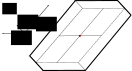
\includegraphics[width=0.5\linewidth]{graphics/zonotope}
  \captionof{figure}{Exemplary creation of a Zonotope $Z$ with $l=2$, $k=3$ and the three generators $p_1,p_2,p_3$.}
  \label{fig:zonotope}
\end{figure}

\end{definition}

When applying the projection $W_r^T$ to the inputs $x \in \Omega$, it holds that
\begin{equation}
\begin{split}
W_r^T x=~W_r^T \sum_{i=1}^d x_i e_i=~\sum_{i=1}^d x_i p_i , ~~~~ p_i=W_r^T e_i
\end{split}
\end{equation}
where the $p_i$ are just the projected unit vectors.
Therefore, since for all components $x_i \in [0,1]$, we can express the transformed inputs with
\begin{equation}
\{W_r^T x \mid x \in \Omega\}=\left\{\sum_{i=1}^d x_i p_i \mid x \in \Omega \right\}=\left\{ \sum_{i=1}^r x_i p_i \mid 0 \leq x_i \leq 1\right\}
\end{equation}
To get closer to the zonotope definition in equation \ref{zonotope}, we first center the inputs $x \in \Omega$ before applying the projection and divide the generators $p_i$ by 2.
Let $c_i=(\frac{1}{2}, \dots, \frac{1}{2})^T\in \mathbb{R}^i$ be the center of the $i$-dimensional hypercube.
Then
\begin{equation}
\begin{split}
&\left\{W_r^T (x - c_d) \mid x \in \Omega\right\}\\
=&\left\{W_r^T \sum_{i=1}^d (x_i - \frac{1}{2}) e_i \mid x \in \Omega \right\}\\
=&\left\{\sum_{i=1}^d (x_i - \frac{1}{2}) W_r^T e_i \mid x \in \Omega \right\}\\
=&\left\{\sum_{i=1}^d (x_i - \frac{1}{2}) q_i \mid x \in \Omega \right\}, ~~ q_i=W_r^T e_i\\
=&\left\{\sum_{i=1}^d (x_i - \frac{1}{2}) q_i \mid 0 \leq x_i \leq 1 \right\}\\
=&\left\{\sum_{i=1}^d x_i p_i' \mid -\frac{1}{2} \leq x_i \leq \frac{1}{2} \right\}\\
=&\left\{\sum_{i=1}^d \frac{1}{2} x_i q_i \mid -1 \leq x_i \leq 1 \right\}\\
=&\left\{\sum_{i=1}^d x_i p_i \mid -1 \leq x_i \leq 1 \right\}, ~~ p_i=\frac{1}{2} q_i
\label{zonotope_form}
\end{split}
\end{equation}

Therefore we define the projection function with
\begin{equation}
p \colon \Omega \mapsto Z, ~~ p(x)=W_r^T (x-c_d)
\end{equation}
This results in a projected input space that has the zonotope form as in equation \ref{zonotope} with
\begin{equation}
Z_{p}=\{\sum_{i=1}^d p_i x_i , ~ -1 \leq x_i \leq 1\}, ~~ p_i=\frac{1}{2} W_r^T e_i
\end{equation}
Then according to equation \ref{zonotope_form}, it holds that $Z_{p}=p(\Omega)$.

\subsection{Surrogate space}

However since the surrogate creation process expects inputs from a $r$-dimensional unit hypercube $\Omega_r$, during the normalization step, the zonotope $Z_p$ is first encased in an $r$-dimensional hypercube called the surrogate space $S$ which is later scaled and aligned to obtain the unit hypercube $\Omega_r$.
To make the generation of the surrogate space easier, the generators $p_i$ of $Z_p$ are ordered by their magnitude.
\todo{Proof that this will result in best possible encasement!}

The generators $q_1, \dots, q_r$ of the encasing hypercube are calculated by applying the Gram–Schmidt process on the ordered zonotope genrators $p_i$ with
\begin{equation}
q_i=p_i - \sum_{k=1}^{i-1} \frac{\langle q_k, p_k\rangle}{\langle q_k, q_k\rangle}
\nonumber
\end{equation}

The surrogate space $S$, which encases the zonotope $Z$, is then an $r$-dimensional hypercube with
\begin{equation}
S=\{\sum_{i=1}^r q_i x_i s_i , ~ -1 \leq x_i \leq 1\},~~ s_i=\sum_{k=1}^d \langle q_i, p_k\rangle
\label{surrogate_space}
\end{equation}
where the scaling factors $s_i$ make the hypercube $S$ exactly match the extent of the zonotope $Z$ as shown in \ref{fig:surrogate_space}.


\begin{figure}[H]
\centering
  \includegraphics[width=0.4\linewidth]{graphics/s}
  \captionof{figure}{Construction of the surrogate space $S$ for the zonotope of figure \ref{fig:zonotope} according to \eqref{surrogate_space}.}
  \label{fig:surrogate_space}
\end{figure}

In theory, the generators $p_i$ that are used to calculate the $q_i$ don't have to be ordered.
However, to improve the generation of the surrogate space, the generators $p_i$ are ordered by their magnitude w.l.og. $|p_1|\geq \dots \geq |p_d|$.
This will improve the surrogate space $S$ in terms of unused space $S \setminus Z$.
\todo{Proove?}


\subsection{Reduced unit hypercube}

The surrogate space $S$ can then be easiliy transformed into a unit hypercube $\Omega_R$ as shown in \ref{fig:aligned} and therefore elements $z \in Z$.
First, by using a change of basis from the unit basis into the surrogate space basis given by the $q_i$.

Let
\begin{equation}
Q=\begin{bmatrix}
  \\
    q_1 ~ q_2 ~ \dots ~q_{r-1} ~ q_r\\
    \\
  \end{bmatrix}
  , ~~
\label{alignment}
\end{equation}
be the new basis matrix.

We can then obtain $u=Q^T z$, where $u_i \in [-s_i,s_i]$ since this is the range of the surrogate space defined in \ref{surrogate_space}.
Once the projected inputs $z \in Z=p(\Omega)$ are represented by the new basis, it is trivial to transform the surrogate space into an $r$-dimensional unit hypercube $\Omega_r$.
First, the $u$ have to be scaled down with
\begin{equation}
u_s=\Gamma u, ~~ \Gamma=\text{diag}(\frac{1}{2 s_1}, \dots, \frac{1}{2 s_r}), ~~
\label{alignment}
\end{equation}
s.t. $(u_s)_i \in [\frac{1}{2},\frac{1}{2}]$.

Then the $u_s$ just have to be translated again from the center away with
\begin{equation}
t_{\text{Cube}}(x)=c_r + u_s = W_r^T (x-c_d)
\end{equation}

\begin{figure}[H]
\centering
  \includegraphics[width=0.4\linewidth]{graphics/s_unit}
  \captionof{figure}{Transformation of $S$ from figure \ref{fig:space} into a unit hypercube according to \eqref{alignment}}
  \label{fig:f2_combined_rel_errors_inter}
\end{figure}


\subsection{Visualizing transformation}

While it is not required to revert the previously shown transformation process, i.e. going from $\Omega_r$ to $\Omega$, later figures in this thesis use the described reversing to illustrate lower dimensional transformed sparse grids in the original and higher-dimensional space.
It is therefore only shown in a more informal way.

\textbf{Inverting the transformation  }
For certain operations it is necessary to invert the transformation.
For this we define the inverse transformation as follows:
\begin{equation}
t^{\text{inv}}(x_{t})=\{x \in \Omega \mid t(x)=x_{t}\}
\end{equation}
In the case of a linear dimensionality preserving transformation, it holds that $|t^{\text{inv}}(x_{t})| \in \{0,1\}$.
Otherwise, we can't infer anything about the cardinality of the inverse, i.e. $|t^{\text{inv}}(x_{t})| \geq 0$.
Luckily there is no need to compute $t^{\text{inv}}(x_{t})$. Instead for conducting operations on the surrogate, it suffices to determine wether a point $x_t \in \Omega_t$ is unused, i.e. $|t^{\text{inv}}(x_{t})| = 0$, which can be done quickly.
\\
\\

Let $y=t_{\text{Cube}}(x)$ be the transformed input. It then holds that
\begin{equation}
x=(W_r Q \Gamma^{-1} (y - c_r)) + c_d
\end{equation}

\begin{figure}[H]
\centering
  \includegraphics{graphics/surrogate_vis}
  \captionof{figure}{Transformation of $S$ from figure \ref{fig:space} into a unit hypercube according to \eqref{alignment}}
  \label{fig:f2_combined_rel_errors_inter}
\end{figure}

\section{Active Subspaces}


The method of active subspaces \cite{CG15} aims to identify the most influential directions in the parameter space to construct a lower-dimensional subspace of $\Omega$ which covers most of a models output variance to conduct parameter studies with a reduced amount of dimensions.
In constrast to conducting parameter studies, we will use the so-called active directions to construct the $W_r$.
Let
\begin{equation}
C = \int_{\Omega} (\nabla f) (\nabla f)^T \rho ~ dx
\label{as_c}
\end{equation}
be the average outer product of the gradient, a $(d \times d)$ matrix.
Since $C$ is a positive semi-definite matrix, it is possible to decompose it into its eigenvectors $v_i$ and their corresponding real eigenvalues $\lambda_i$ with
\begin{equation}
C = V \Lambda V^T, ~~ \Lambda = diag(\lambda_1, ..., \lambda_d), ~~ V=
  \begin{bmatrix}
  \\
    v_1 ~ v_2 ~ \dots ~ v_{d-1} ~ v_d\\
    \\
  \end{bmatrix}
\nonumber
\end{equation}

We furthermore assume that the eigenvectors in this decomposition are ordered, i.e. $\lambda_1 \geq ... \geq \lambda_d$.
A larger eigenvalue indicates a higher rate of change along the direction, more precisely it is the average squared directional derivative of f with respect to its eigenvector $v_i$ \cite{CG14} with
\begin{equation}
\lambda_i=\mathds{E}[((\nabla f)^T v_i)^2]
\label{eigenvalues}
\end{equation}
Therefore, the column vectors of the matrix $V$ are ordered from most the active direction $v_1$ to least the active direction $v_d$.
By keeping only a specific amount of the most active directions $r \leq d$ we obtain
\begin{equation}
W_r=\begin{bmatrix}
  \\
    v_1 ~ v_2 ~ \dots ~ v_{i-1} ~ v_r\\
    \\
  \end{bmatrix}
\label{basis}
\end{equation}

In the context of this thesis, the given input sample $S$ is used to derive the matrix $C$ from \ref{as_c} using a classical Monte-Carlo approach.
The matrix $C$ can then be approximated with
\begin{equation}
C \approx \frac{1}{n} \sum_{i=1}^n  (\nabla f(y_i)) (\nabla f(y_i))^T
\nonumber
\end{equation}




\subsection{Estimating gradients for Active Subspaces}

If the gradient function is not known and can not be calculated analytically, the gradients can be approximated in various ways.
There are various different methods of achieving that, however each method has its advantages and disadvantages as will be showcased in this section.

\begin{definition}[$L^2$ norm]
Let $v \in \mathds{R}^{n}$ be a vector. Then
\begin{equation}
\| v\|_2=\sqrt{\sum_{i=1}^n |v_{i}|^2}
\nonumber
\end{equation}
is the $L^2$ norm of the vector $v$.
\end{definition}

To judge the quality of approximated gradients, we first have to define an error metric for them.

\begin{definition}[Average gradient error]
Let $S=\{x_1, \dots, x_n\}$ be a sample and $\widetilde{\nabla f(x_i)}$ the approximated gradient at sample point $x_i$. Then
\begin{equation}
e_{\text{grad}}(S)=\frac{1}{n} \sum_{i=1}^n \frac{\| \widetilde{\nabla f(x_i)} - \nabla f(x_i) \|_2}{\| \nabla f(x_i) \|_2}
\nonumber
\end{equation}
is the average gradient approximation error of the sample.
\end{definition}

The approximated gradients are then used as inputs for equation \ref{} to obtain the approximated Active Subspace matrix.

\begin{definition}[Frobenius norm]
Let $A \in \mathds{R}^{m \times n}$ be a matrix. Then
\begin{equation}
\| A\|_2=\sqrt{\sum_{i=1}^m \sum_{j=1}^n |a_{i,j}|^2}
\nonumber
\end{equation}
is the Frobenius norm of the matrix $A$.
\end{definition}

The most basic error metric for an estimated Active Subspace matrix would be calculating the Frobenius norm of the approximation error, i.e. $\| V - V^* \|_2$.
However, this error calculation is not suitable for cases in which $\lambda_i \approx 0$, since the corresponding eigenvector can vary greatly in that case.
It has therefore to be adapted for example by omitting the affected eigenvectors from the calculation if such a case occurs.
I.e. we have to input a matrix of eigenvectors where the active directions with $\lambda_i \approx 0$ are already eliminated.

\begin{definition}[Active Subspace error]
Given an estimated Active Subspace eigenvector matrix $W_r$ and the reference eigenvector matrix $W_r^*$, the
Active Subspace error is calculated with
\begin{equation}
e_{\text{AS}}(W_r)=\frac{\| W_r - W_r^* \|_2}{\| W_r^* \|_2}
\nonumber
\end{equation}
\end{definition}

In the context of Active Subspaces, the approximation error of the gradients is not the relevant metric to evaluate a method.
Instead, the primary focus is the Active Subspace approximation error, which is decoupled from the individual gradients, since it is based on the average outer product of the gradients.
While the individual gradients approximated by different methods can be far off, the gradient average can still come close to the real one if the general trend of the gradients is still be reflected with the method.
Therefore, inaccuracies of single gradients can be averaged out but systematic biases of the gradients will influence the Active Subspace.


\subsection{Finite differences}

The most common approach to estimate the gradients are finite differences.
In this thesis, an adaptive mix of forward and backward differences are used with a fixed distance $h$ where the range of possible distance is defined by $0 < h \leq 0.5$ such that
\begin{equation}
\frac{\partial f(x)}{\partial x_i} \approx
\begin{cases}
    \dfrac{f(x_1, \dots, x_i + h, \dots, x_d) - f(x)}{h}, & x_i + h \leq 1 \\[1.5em]
    \dfrac{f(x_1, \dots, x_i - h, \dots, x_d) - f(x)}{h}, & \text{else}
\end{cases}
\end{equation}

The downside in the context of the sample-based approach is the requirement to additionally evaluate the model function at $d$ other inputs to determine the gradient at one sample point.
For high $d$ and a large amount of samples $n$, $dn$ function evaluations for finite differences may become too costly.
Alternatively, the gradients can be determined using a different approach that only works on a given input sample and does not require other function evaluations.

\subsection{Directional derivatives}

Another approach is to roughly approximate the gradient by looking at neighboring points in the same sample and using directional derivatives to create a system of linear equations for the gradient at a certain input.
Given two inputs $x, y \in \Omega, x \neq y$, we define the distance between the two inputs as $r=y-x$.
By extrapolating the gradient along the direction in a linear fashion, we can define an approximation rule with
\begin{equation}
r \nabla_x f \approx f(y) - f(x)
\end{equation}

Using $m \in \mathds{N}$ neighbours of a sample point $x \in \Omega$ with $y_i \in \Omega \setminus \{x\}, ~ i \in \{1, \dots, m\}$, we can create a system of linear equations with
\begin{equation}
\begin{bmatrix}
    y_1 - x\\
    \vdots \\
    y_m - x
  \end{bmatrix}  \nabla_x f =\begin{bmatrix}
    f(y_1) - f(x) \\ \vdots \\  f(y_m) - f(x)
    \\
  \end{bmatrix}
  \label{dd_sle}
\end{equation}

One limitation of this calculation is the linear nature of the calculated gradients, i.e. estimating gradients of a non-linear function can lead to biased gradients.
Furthermore, the choice of the $y_i$ heavily influences the result as well as the size of $m$.
The next sections introduce different ways of selecting the neighbours $y_i$ and also evaluate the results.

\subsection{Random neighbour approximation}

The random neighbour approximation method takes as an input a subsample $S_{\text{rn}} \subseteq S \setminus \{x\}$ with $|S_{\text{rn}}|=m < n$.
The set $S_{\text{rn}}=\{y_1, \dots, y_{m}\}$ is called a random neighbour set of $x$.
This random neighbour set is then used as an input for equation \ref{dd_sle} to approximate the gradient $\nabla_x f$.

For $n,m \to \infty$, the approximated gradient does not converge to the actual gradients, since the expected distance to the neighbours in a random neighbour set does not go to zero.
The problem of determining average neighbour distance is related to finding the mean line segment length $\Delta (d)$ in a d-dimensional unit hypercube \cite{}.
There is no closed form solution for $\Delta (d)$, but several approximations have been made \cite{}, e.g. $\Delta (1)=\frac{1}{3}$, $\Delta (2)=0.52$, $\Delta (3)=0.66$.

\subsection{Nearest neighbour approximation}

The nearest neighbour variant picks a subset $S' \subseteq S \setminus \{x\}$ with a manageable size $n'=|S'|$ similar the the random neighbour method and then calculates the $m \leq n'$ nearest neighbours $S_{\text{nn}}=\{y_1,\dots,y_m\} \subset S'$ of the point $x$ with $|(y_1-x)| < |(y_2-x)|< \dots<|(y_{m-1}-x)| < |(y_{m}-x)|$.

Compared to the random neighbour approximation, for $n,n',m \to \infty$, the approximated gradient does converge to the actual gradient, since the expected distance to the neighbours does go to zero.
However, this property comes at the cost of having to sort the available $n'$ neighbours by distance to pick the $m$ closest ones.
The parameters $n'$ and $m$ also have to be chosen carefully, as a too low ... and a too large $m$ would increase the average distance to the neighbours again so that the effect of chosing the nearest neighbours would diminish.


\begin{figure}
\begin{subfigure}{.5\textwidth}
  \centering
  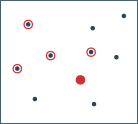
\includegraphics[width=.8\linewidth]{graphics/as_rn}
  \caption{Random neighbour method with $m=4$}
  \label{fig:as_rn}
\end{subfigure}%
\begin{subfigure}{.5\textwidth}
  \centering
  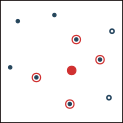
\includegraphics[width=.8\linewidth]{graphics/as_nn}
  \caption{Nearest neighbour method with $n'=7$ and $m=4$}
  \label{fig:as_nn}
\end{subfigure}
\caption{Differences in sample selection between the two neighbour approximation methods. The red circle represents the sample point $x$, the black dots are the other available samples $S \setminus \{x\}$. In this example $|S|=10$. A filled black dot signals that it is considered when looking for neighbours. If the circle is circled blue, it is chosen as a neighbour.}
\label{fig:as_approx}
\end{figure}

\subsection{Approximation quality}

To get an idea of the actual quality of the different methods, this section will focus purely on the gradient approximation methods as a ... before the methods are used in the surrogate creation process later on.
Two example functions are investigated with the focus being on first the gradient approximation quality and the subsequent Active Subspace approximation quality.

\newpage

\subsection{Simple function}

The first example function is a simple $3$-dimensional function with two-dimensional polynomial terms:
\begin{equation}
f_1(x)=(0.8 {x_1}^2 - x_2) / (x_3 + 0.5)
\nonumber
\end{equation}



\begin{figure}[H]
\begin{center}
	\includegraphics[width=\textwidth]{graphics/as_errors_f1}
\end{center}
	\captionof{figure}{Mean Active Subspace error calculated with the previously introduced methods compared to the actual Active Subspace for $f_1$ over 10 iterations .}
	\label{fig:as_errors_f1}
\end{figure}

As seen on the left in figure \ref{fig:as_errors_f1}, the finite differences approximation error converges towards zero as the step size goes down as expected.
Furthermore, the nearest neighbour method does deliver better results than the random neighbour method.
The random neighbour methods do not converge but are instead in a range that is even worse compared to the finite differences approximation with a very big step size.
Since the mean line segment length is $\Delta(3) \approx 0.66$, the random neighbour method chooses on averages neighbours with a distance $|d| \approx 0.66$.
It can be seen that the average gradient error for all $RN$ methods is a little bit worse than FD with $h=0.5$, which is consistent with the average distance differences between the two methods.

As a result of the approximation qualities shown on the right in figure \ref{fig:as_errors_f1}, the gradient approximation qualities behave similar.
The random neighbour methods are still in a small range with an error comparable to the finite differences approximation with a very big step size of $h=0.5$.
The nearest neighbour method does deliver far better results than the random neighbour method, as it shows a similar quality as the finite differences approximation with smaller step sizes.
Also, using fewer closer neighbours $m$ for the nearest neighbour method seems to be better.
It can also be observed that the gradient approximation quality does not completely correlate with the Active Subspace approximation quality.
While for example the $NN$ methods have a similar gradient approximation quality as $FD$ with $h=0.1$, the $NN$ calculated Active Subspaces have a far better quality than the $FD$ with $h=0.1$.

\newpage

\subsection{Complex function}

The second case study is a 20-dimensional function:

\begin{align}
\begin{split}
f_2(x_0, \dots, x_{19})=&e^{0.2 x_0 x_1 x_2 x_3 x_4}\\
+ &5 * sin(\pi x_5 x_6 x_7) x_8^2 x_9^5 x_{10}\\
+ &(x_{11} + 2)^2 x_{12}\\
+ &2 x_{13} * 3 x_{14}\\
+ &x_{15} x_{16}\\
+ &log(1 + (10 x_{17} / (0.1 + x_{18} + x_{19})))
\end{split}
\end{align}

\begin{figure}[H]
\begin{center}
	\includegraphics[width=\textwidth]{graphics/as_grad_errors_f2}
\end{center}
	\captionof{figure}{Average $L^2$ error of gradients calculated with the previously introduced methods compared to the actual gradients for $f_2$.}
	\label{fig:as_grad_errors_f2}
\end{figure}

As seen in figure \ref{fig:as_grad_errors_f2}, the finite differences approximation error converges towards zero as the step size goes down as expected.

\begin{figure}[H]
\begin{center}
	\includegraphics[width=\textwidth]{graphics/as_errors_f2}
\end{center}
	\captionof{figure}{Mean Active Subspace error calculated with the previously introduced methods compared to the actual Active Subspace for $f_2$ over 10 iterations .}
	\label{fig:as_errors_f2}
\end{figure}

...

\section{Random linear transformations}

A completely different approach to finding a transformation function is just generating a random one.
A random transformation generator is easy to implement, can generate new transformation functions almost instantly and offers a purely exploratory approach to finding the best transformation.
It can also serve as a reference for comparision as one would expect that the Active Subspace method should always output better transformation.

Generating uniformly distributed orthonormal matrices is not trivial, but important when generating many of them to avoid any generation bias.
\cite{ABC} presents an algorithm to generate unitary matrices and also a slightly modified version to uniformly generate elements from the orthogonal group $O(d)$.
It starts off with generating a random matrix $Z$ with $z_{i,j} \sim \mathcal{N}\left(0, 1\right)$.
The matrix $Z$ is then fed into a $QR$ decomposition with $Z=QR$.
The entries of the diagonal matrix $R$ are then normalized to get
\begin{equation}
\Lambda=\text{diag}\left(\frac{r_{1,1}}{|r_{1,1}|}, \dots, \frac{r_{d,d}}{|r_{d,d}|}\right)
\end{equation}
The matrix $W=Q \Lambda Q$ is then uniformly distributed with Haar measure, i.e. exactly what we are looking for.


\section{Other transformations}

Until now, the focus was primarily on linear transformations because they are relatively easy to construct.
However, in theory one can use arbitrary transformation functions.

\subsection{Periodic transformations}

Another use case for transformations are periodic functions.
If the model function $f$ is for example periodic along one dimension $i$, i.e. $f(x_1,\dots,x_i,\dots,x_d)=f(x_1,\dots,x_i\text{ mod } h, \dots,x_d)$, we can easiliy define a transformation with $t(x_1,\dots,x_i,\dots,x_d)=(x_1,\dots,(x_i\text{ mod } h) /h, \dots,x_d)^T$ and create a surrogate with $f(x) \approx \hat{f}(t(x))$.
This way, the function can be interpolated better because there are effectively $1 / h$ times more grid points spent along the $i$-th dimension.
Of course this can concept can be expanded upon with multiple periodic dimensions, antiperiodic functions, offsets and combination with linear transformations.

\todo{Example with $f(x)=sin(2\pi x_1) x_2^2$}

\subsection{Active Manifolds}

Inspired from Active Subspaces, which are purely linear in their nature, one can extend the concept to identifying a one-dimensional curve in the domain $\Omega$ along the flow of most active change, which is called the Active Manifold.
Compared to Active Subspaces, calculating the Active Manifold is more complex and resource intensive.
Furthermore, defining a transformation function that maps from $\Omega$ onto the local one-dimensional space of the curve is way more complex and can be constructed in many ways.
Also they are currently limited to one dimension, for which the surrogate construction method becomes pretty irrelevant.


\chapter{Surrogates for transformations}

Once a transformation function $t(x)$ has been created, the next step is creating a surrogate for the transformed input space $\Omega_r=t(\Omega)$.
The original inputs $y_i \in S$, which were drawn randomly according from the pdf $\rho$, are transformed to obtain the transformed sample $S_r=t(S)$ where the $z_i \in S_r$ transformed inputs with $z_i \in \Omega_r$.
There are many different ways of constructing the surrogate $\hat{f}_r$.
The approach used here is function regression with spatially adaptive sparse grids as described in \cite{P10} where $m \leq n$ samples are used to create an approximation of the model function.
We are aiming to construct the function $\hat{f}_r$ using spatially adaptive sparse grids and an arbitrary basis , i.e.
\begin{equation}
\hat{f}_r(x) \coloneqq \sum_{\underline{l},\underline{i}} \alpha_{\underline{l},\underline{i}} \phi_{\underline{l},\underline{i}}(x)
\end{equation}

The dataset used for the regression is then defined as
\begin{equation}
\{(t(y_i),f(y_i)), ~ y_i \in S, ~ 1 \leq i \leq m\}
\end{equation}
Thus, we are trying to solve the least squares problem with the standard square loss function for the dataset $S$ with
\begin{equation}
\epsilon(\hat{f}_r)=\frac{1}{m} \sum_{i=1}^m (f(y_i) - \hat{f}_r(t(y_i)))^2 
\end{equation}

Note that this data might be, depending on the model to reduce, very noisy and there even might be multiple different values for the same inputs, i.e. $(y_i,f(y_i)), (y_j,f(y_j)) \in S, ~ y_i=y_j, f(y_i) \neq f(y_j)$.
Since the surrogate construction is usually an ill-posed problem and we are calculating a regressed function only based on the samples $S$, the regression method used employs regularization as well to prevent overfitting.
We are therefore solving the regularized least squares problem with the smoothing factor $\lambda > 0$:
\begin{equation}
\hat{f}_r^{\lambda^*} = \argmin_{\hat{f}_r^\lambda \in V} \epsilon_{S}(\hat{f}_r^\lambda) + \lambda R(\hat{f}_r^\lambda)
\end{equation}

\section{Multifidelity surrogates}

The construction of the best possible Sparse Grid surrogate, given inputs, a transformation, and set of possible configuration parameters can become very computationally expensive, since every parameter combination has to be evaluated.
To mitigate this problem, we employ the concept of multifidelity simulations \cite{}, i.e. reducing the cost of parametrization by using low fidelity Sparse Grids and datasets to evaluate a parameter combination and only using high fidelity Sparse Grids and datasets when creating the final surrogate using the determined to be optimal parameters.

A low fidelity Sparse Grid surrogate $\hat{f}^l$ has less grid points compared to an otherwise identical high fidelity Sparse Grid surrogate $\hat{f}^h$.
This means that the level of $\hat{f}^l$ is lower and less or not refinements at all are used.
It is vital that the used low fidelity surrogates still stay representative when comparing the errors for different parameter combinations.
They don't have to be representative of the high fidelity surrogate error, but should fullfil the following property:
\begin{equation}
\epsilon(\hat{f}_1^l) < \epsilon(\hat{f}_2^l) \Rightarrow \epsilon(\hat{f}_1^h) < \epsilon(\hat{f}_2^h)
\end{equation}
i.e. they should be indicative of the comparative quality of their high fidelity surrogates.

This multifidelity approach will also be used in later chapters in a more extended fashion to also evaluate multiple different transformations to choose the best one.
As already mentioned, the ability to evaluate transformations is critical for the random transformation method \ref{}, as it allows for the generation and evaluation of many more transformation to choose the best from.

\section{Operations on transformed surrogates}

Now that a surrogate has been created and we can approximate the model function with $f(x) \approx \hat{f}_r(t(x))$,
we can look at the differences when using transformed surrogates compared to the standard case of directly approximating the model function with $f(x) \approx \hat{f}(x)$ and not using a transformation.

\textbf{Differentiation }
Assuming that the surrogate uses a basis that can be differentiated easily, such as B-Splines, the gradient can be approximated using the chain rule and the gradient function of the transformed surrogate with
\begin{equation}
\nabla f(x) \approx \nabla \hat{f}_t(t(x)) = \nabla (\hat{f}_t \circ t)(x)=(Dt(x))^T \nabla \hat{f}_t(t(x))
\end{equation}
\\
\\
\textbf{Inverting the transformation  }
For certain operations it is necessary to define the inverse of the transformation function.
For this we define the inverse transformation as follows:
\begin{equation}
t^{\text{inv}}(x_{t})=\{x \in \Omega \mid t(x)=x_{t}\}
\end{equation}
In the case of a linear dimensionality preserving transformation, it holds that $|t^{\text{inv}}(x_{t})| \in \{0,1\}$.
Otherwise, we can't infer anything about the cardinality of the inverse, i.e. $|t^{\text{inv}}(x_{t})| \geq 0$.
Luckily there is no need to compute $t^{\text{inv}}(x_{t})$. Instead for conducting operations on the surrogate, it suffices to determine wether a point $x_t \in \Omega_t$ is unused, i.e. $|t^{\text{inv}}(x_{t})| = 0$, which can be done quickly.
\\
\\
\textbf{Transformed distribution}
The input probability distribution $\rho \colon \Omega \to \mathds{R_+}$ with $\int_{\Omega} \rho \; \text{d}x = 1$ also changes for the transformation surrogate.
We define the transformed distribution as
\begin{equation}
\rho_r \colon \Omega_r \to \mathds{R_+}, ~~ \rho_r(x_r)=\int_{t^{\text{inv}}(x_r)} \rho(x) \; \text{d}x 
\end{equation}
This is also a distribution since it holds that
\begin{equation}
\int_{\Omega_r} \rho_r(x_t) \; \text{d}x=\int_{x_r \in \Omega_r} \int_{t^{\text{inv}}(x_r)} \rho(x) \; \text{d}x = \int_{\Omega} \rho(x) \; \text{d}x = 1
\end{equation}
This means that in many cases for example a uniform distribution $\rho$ will be transformed into a non-uniform distribution $\rho_r$.
\\
\\
\textbf{Density Quadrature}
Given an input distribution $\rho$ and transformation $t$, we can compute the integral with
\begin{equation}
\int_{\Omega} f(x) \rho(x) \; \text{d}x \approx \int_{\Omega} \hat{f}_t(t(x)) \rho(x) \; \text{d}x
=
\int_{\Omega_r} \hat{f}_t(z) \left(\int_{t^{\text{inv}}(z)} \rho(x)  \; \text{d}x \right)  \; \text{d}z=
\int_{\Omega_r} \hat{f}_t(z) \rho_t(z) \; \text{d}z
\end{equation}
By introducing a transformation we lose the ability to easily use Sparse Grid based quadrature algorithms.
However, since $r$ is usually smaller than $d$, Monte-Carlo based quadrature becomes a better option for transformed surrogates.
\\
\\
\textbf{Quadrature}
Given a transformation $t$, we can easily compute $\int_{\Omega} f(x) \; \text{d}x$ using the surrogate, since it is a special case of density quadrature with $\rho=\mathcal{U}(0,1)^d$.
Even though the original input is uniformly distributed, the resulting surrogate distribution $\rho_r$ is usually not.
\\
\\
\textbf{Optimization}
To calculate the maximum $x^\text{max} \coloneqq \argmax_{x \in \Omega} f(x)$ or minimum $x^\text{min} \coloneqq \argmin_{x \in \Omega} f(x)$ of the model function, one can also optimize the surrogate. There exist many different algorithms, especially for B-Spline basis functions presented in \cite{}.
After having applied a transformation, there might unused points $x_r \in \Omega_r$ in the surrogate space, i.e. $\nexists x \in \Omega \colon t(x)=x_r$.
Therefore a constrained optimization has to be performed on the surrogate first with
\begin{equation}
x_{r}^\text{max} \coloneqq \argmax_{x_r \in \Omega_r} \hat{f}(x_r), ~ |t^{\text{inv}}(x_{r})|\geq 1
\end{equation}
Afterwards, at least in the dimensionality preserving transformation, we can obtain the maximum $x^\text{max}$ with $x^\text{max}=t^{\text{inv}}(x_{r}^\text{max})$, since $|t^{\text{inv}}(x_{r}^\text{max})|=1$.
One problem is that in the case of a reducing transformation with $r<d$, a computed surrogate maximum $x_{r}^\text{max}$ may be a set of many points.
Therefore another non sparse grid based optimization can be performed on the set $t^{\text{inv}}(x_{r}^\text{max})$, to get a good maximum estimate.

\chapter{Algorithm}

We now covered all the tools needed to approximate the model function with a transformed surrogate.
However, we can take a look at similar methods and take some inspirations from them.
One of these related methods is projection pursuit regression \cite{}.

\section{Projection pursuit regression}

The projection pursuit regression method comes from the area of statistics and is in its core idea related to our approach with linear transformations.
It tries to represent a dataset $P=\{(x_i, y_i)=(x_i, f(x_i))\}$ using the form
\begin{equation}
y_i=\beta_0 + \sum_{i=1}^m f(\beta_i^T x_i) + \epsilon_i
\end{equation}
where $\beta_0$ is a constant, $\beta_i$ are ..., and the $\epsilon_i$ are the residiuals.
Using the $\beta_i$ to project inputs onto a lower-dimensional hyperplane is very similar to our concept of creating linear transformations.


Going from this statistical model to our function approximation problem, we can 
\begin{equation}
f(x)=\sum_{i=1}^m f(\beta_i^T x_i)
\end{equation}
The functions $\hat{f}_i$ and projections $\beta_i$ of this additive model can be calculated iteratively by applying one step of finding a projection and constructing a surrogate repeatedly each time on the error function
\begin{equation}
e_k(x)=f(x) - \sum_{i=1}^k f(\beta_i^T x_i)
\end{equation}

\begin{algorithm}[H]
\normalsize
\begin{algorithmic}
\Function{projectionPursuitRegression}{$f, m$}
    \State $e_0 = f$
    \For{$i = 1, \dots, m$}
    	\State $\beta_i \gets$ best
    	\State $e \gets e_{i - 1} - \hat{f}_i$
    \EndFor
    \State $\hat{f} \gets \sum_{i=1}^m f(\beta_i^T x_i)$
    \State \Return{$\hat{f}$}
\EndFunction
\end{algorithmic}
	\captionof{algorithm}{Pseudocode of the iterative projection pursuit regression algorithm. Alternatively, one could introduce an error exit condition that exists the loop if the regression error is small enough with $\epsilon(e) < \epsilon_{max}$.}
\end{algorithm}

\todo{Mean center function?}

\section{An iterative approach}

\begin{algorithm}[H]
\normalsize
\begin{algorithmic}
\Function{transformedSurrogateSum}{$f, m$}
    \State $e_0 = f$
    \For{$i = 1, \dots, m$}
    	\State $t_i \gets$ generateBestTransformation()
    	\State $\hat{f}_{t_i,i} \gets$ generateBestSurroate($t_i$)
    	\State $e \gets e_{i - 1} - \hat{f}_{t_i,i}$
    \EndFor
    \State $\hat{f} \gets \sum_{i=1}^m \hat{f}_{t_i, i} \circ t_i$
    \State \Return{$\hat{f}$}
\EndFunction
\end{algorithmic}
	\captionof{algorithm}{Pseudocode of the iterative projection pursuit regression algorithm. Alternatively, one could introduce an error exit condition that exists the loop if the regression error is small enough with $\epsilon(e) < \epsilon_{max}$.}
\end{algorithm}

In the case that we use a linear transformation function, the algorithm is pretty much identical to the previous one.

\section{Determining the best transformation and surrogate}

T

\todo{local vs global optimization}


\section{Visualizing the algorithm}

\chapter{Implementation}

To make the shown results as transparent as possible, this chapter will focus on how the previsouly described process of transforming Sparse Grids is actually implemented.

\begin{description}
\item[Object] An object can represent any kind of data, for example a model function, a function sample, a transformation function, a surrogate, and more.
\item[Function] A function takes optional inputs in the form of objects, performs some kind of operation, and outputs an object.
\item[Component] A component is a function declaration, where the actual implementation can be exchanged for many different function implementations.
\item[Control flow + data flow] Arrows signal control flow and also data flow if an object is shown.
\end{description}

\begin{figure}[H]
\includegraphics[width=\textwidth]{graphics/definitions.pdf}
\captionof{figure}{Notation used for different elements in the structure diagrams.}
\label{fig:defs}
\end{figure}

Functions and components can also be customized by passing some configuration parameters, which is not explicitly shown in the structure diagrams but will be mentioned if it is done.

\newpage
\section{Pipeline}

The whole reduction process is modeled and implemented as a pipeline made up of different components to allow for maximum flexibility.
All components can be exchanged for many different types, where instances of these types can also be customized by passing some configuration parameters.

\begin{figure}[H]

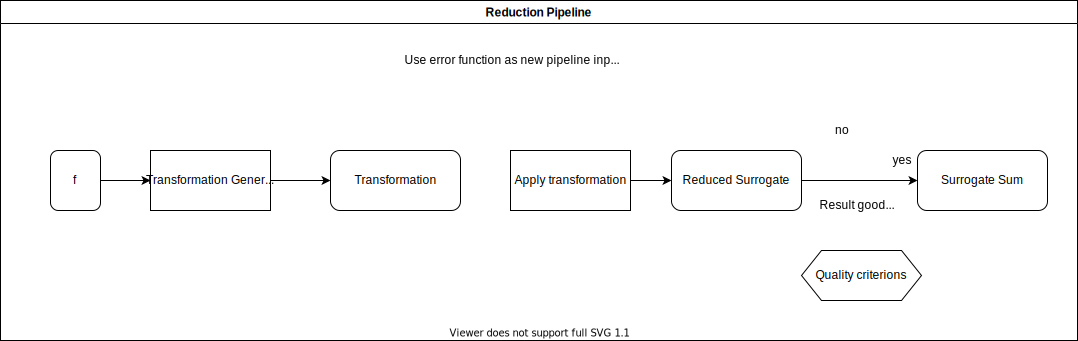
\includegraphics[width=\textwidth]{graphics/ReductionPipeline.pdf}
\vspace{-1.5mm}

\begin{mdframed}[linewidth=0.7px]

\begin{description}
\item[Parameters] {~ \begin{enumerate}[\indent{}]
\item \texttt{\textbf{numIterations}}: Maximum amount of iterations
\item \texttt{\textbf{functionSample}}: A sample
\end{enumerate}}
\end{description}

\end{mdframed}
\captionof{figure}{Component structure of the transformation pipeline and the associated possible configuration options.}
\label{fig:astsg}
\end{figure}

The core component of the reduction pipeline and also the most important one wrt. achieving good reduction results in the transformation function generator.

\newpage
\section {Transformation generators}
\label{sec:tg}

The transformation generator component has the responsibility of finding a good transformation function to use for a pipeline iteration.

\subsection {Transformation stream generator}

Chapter \ref{} covered the used transformation generation methods in detail.
It described that for every calculated Active Subspace matrix or random orthogonal basis, family of transformations can be generated from them, usually accomplished by using different values for the reduced dimension $r$, i.e. cutting less or more dimensions off.
To apply this concept and couple it with other components, such as transformation evaluators, this implementation makes use of so-called transformation generator streams.
A transformation stream generator will generate as much different transformations as it can, where the range of possible transformations is defined by multiple specific parameters.
It can be parallelized.
Every transformation that is generated from the stream is evaluated using a transformation evaluator and the best transformation will be chosen and returned in the end.

\begin{figure}[H]
\includegraphics[width=\textwidth]{graphics/TransformationGen_Stream.pdf}
\captionof{figure}{Component structure of a stream-based transformation generator and the associated possible configuration options.}
\end{figure}

\newpage

\subsection{Active Subpsace stream generator}

The already described Monte-Carlo Active Subspace method presented in \ref{sec:as} is implemented as a transformation stream generator component as seen in figure \ref{fig:astsg} , since there are multiple different cutoff possibilities.
The exact range of the cutoff dimensions can be customized using various parameters as seen in figure \ref{fig:astsg}.

\begin{figure}[H]

\includegraphics[width=\textwidth]{graphics/TransformationStreamGen_AS.pdf}

\vspace{-1.5mm}

\begin{mdframed}[linewidth=0.7px]

\begin{description}
\item[Parameters] {~ \begin{enumerate}[\indent{}]
\item \texttt{\textbf{maxSampleCount}}: The maximum amount of samples used to create a gradient sample and that is subsequentially passed down to create the Active Subspaces.
\item \texttt{\textbf{minDimensions}}: The minimum amount of used eigen vectors, i.e. the lower bound for $r$.
\item \texttt{\textbf{maxDimensions}}: The maximum amount of used eigen vectors, i.e. the upper bound for $r$.
\item \texttt{\textbf{minEigenValueShare (= 0)}}: Defines a lower bound on the possible values of $r$ by requiring that it holds that $\sum_{i=1}^r \lambda_i / \sum_{i=1}^d \lambda_i \geq \texttt{minEigenValueShare}$.
\end{enumerate}}
\end{description}

\end{mdframed}
\captionof{figure}{Component structure of an Active Subspace transformation stream generator and the associated possible configuration options.}
\label{fig:astsg}
\end{figure}

The Monte-Carlo Active Subspace method requires gradient samples as inputs.
So for a gradient sample generator, four variants can be chosen depending on given inputs and requirements:
\begin{description}
\item[\texttt{\textbf{givenGradient()}}:] If the gradient function of the model function $f$ is known or easy to calculate analytically, then generating a gradient sample is straightforward by just evaluating the gradient function at the sample points.
\item[\texttt{\textbf{finiteDifferences($h$)}}:] Alternatively, the sample gradients can be determined using finite differences if the runtime cost of $d$ model function evaluations per sample point is acceptable.
\item[\texttt{\textbf{randomNeighbour($n'$)}}] Random neighbour approximation according to \ref{}.
\item[\texttt{\textbf{nearestNeighbour($n', m$)}}] Nearest neighbour approximation according to \ref{}.
\end{description}

\newpage

\subsection {Random stream generator}

A completely different approach to finding a transformation function is just generating a random one.
A random transformation generator is easy to implement, can generate new transformation functions almost instantly and offers a purely exploratory approach to finding the best transformation.
It can also serve as a reference for comparision as one would expect that the Active Subspace method should always output better transformation.

\begin{figure}[H]

\includegraphics[width=\textwidth]{graphics/TransformationStreamGen_Random.pdf}

\vspace{-1.5mm}

\begin{mdframed}[linewidth=0.7px]

\begin{description}
\item[Parameters] {~ \begin{enumerate}[\indent{}]
\item \texttt{\textbf{minDimensions}}: The minimum amount of used basis vectors, i.e. the lower bound for $r$.
\item \texttt{\textbf{maxDimensions}}: The maximum amount of used basis vectors, i.e. the upper bound for $r$.
\end{enumerate}}
\end{description}

\end{mdframed}
\captionof{figure}{Component structure of an random transformation stream generator and the associated possible configuration options.}
\label{fig:rtsg}
\end{figure}

\newpage

\subsection {Iterative transformation generator}

In some cases, especially when dealing with a random transformation generation as shown in \ref{sec:rtg}, the probability of finding a good transformation in one try is very low, it makes sense to also introduce an iterative transformation generator component, which can be combined with any other transformation generator component, e.g. a stream-based one.
It can therefore also be used with the Active Subspace transformation generator to try to find the best transformation out of several Active Subspace calculations with different input samples.

\begin{figure}[H]
	\includegraphics[width=\textwidth]{graphics/TransformationGen_Iterative.pdf}

\vspace{-1.5mm}

\begin{mdframed}[linewidth=0.7px]

\begin{description}
\item[Parameters] {~ \begin{enumerate}[\indent{}]
\item \texttt{\textbf{numIterations}}: Iterative transformation generator configuration options
\end{enumerate}}
\end{description}

\end{mdframed}
\captionof{figure}{Component structure of an iterative transformation generator and the associated possible configuration options}
\end{figure}

\newpage
\section {Evaluators}

\subsection {Surrogate evaluator}

The role of a transformation evaluator is to take a newly constructed transformation $t(x)$, evaluate its quality and make it comparable to other transformations.
This is used for iterative and stream-based transformation generators and by the pipeline.
While this is a pretty straightforward process, it can still be customized by changing the surrogate construction rules and error metric.

\begin{figure}[H]
\includegraphics[width=\textwidth]{graphics/SurrogateEval.pdf}
\vspace{-4.5mm}
\begin{mdframed}[linewidth=0.7px]
\begin{description}
\item[\texttt{\textbf{errorMetric}}:] Common error metrics used in this thesis include MSE, RMSE, and NRMSE.
Additionally, penalty terms for various features can be introduced, such as a penalty term that grows with the amount of reduced dimensions of the transformation.
\end{description}
\end{mdframed}
\end{figure}

\subsection {Transformation evaluator}

The role of a transformation evaluator is to take a newly constructed transformation $t(x)$, evaluate its quality and make it comparable to other transformations.
This is used for iterative and stream-based transformation generators and by the pipeline.
While this is a pretty straightforward process, it can still be customized by changing the surrogate construction rules and error metric.

\begin{figure}[H]
\includegraphics[width=\textwidth]{graphics/TransformationEval.pdf}
\vspace{-1.5mm}
\end{figure}

\newpage
\section {Surrogate generator}

The role of a transformation evaluator is to take a newly constructed transformation $t(x)$, evaluate its quality and make it comparable to other transformations.
This is used for iterative and stream-based transformation generators and by the pipeline.
While this is a pretty straightforward process, it can still be customized by changing the surrogate construction rules and error metric.


\subsection {Sparse Grid surrogate generator}

In the case of Sparse Grid surrogates, as used in this thesis, the construction parameters contain all required inputs like grid type, basis functions, level, adaptivity properties, and more.
As runtime performance is important, especially when using evaluators with the iterative transformation generator, finding the right Sparse Grid level ...

\begin{mdframed}[linewidth=0.7px]
\begin{description}
\item[Parameters] {~ \begin{enumerate}[\indent{}]
\item \texttt{\textbf{gridType}}: Type of basis functions according to \ref{}
\item \texttt{\textbf{basisType}}: Type of basis functions according to \ref{}
\item \texttt{\textbf{approxGridPoints}}: Type of basis functions according to \ref{}
\item \texttt{\textbf{maxTrainSamples}}: Type of basis functions according to \ref{}
\item \texttt{\textbf{trainData}}: Type of basis functions according to \ref{}
\item \texttt{\textbf{lambdas}}: Type of basis functions according to \ref{}
\item \texttt{\textbf{refinements}}: Type of basis functions according to \ref{}
\end{enumerate}}
\end{description}
\end{mdframed}

\subsection {RBF surrogate generator}

\chapter{Implementation and evaluation}

\begin{enumerate}
\item How much do different AS transofmrations influence the result?
\end{enumerate}

The goal is to answer the following questions:

\begin{enumerate}
\item What is a good amount of samples? How do different sampling techniques influence the results?

\item How good is the quality of the computed $A_k$ for a certain amount of samples? We compare the errors that occur when using the optimal $A_k$ and the computed $A_k$.

\item How much does a certain deviation of the $A_k$ effect the interpolation error?

\item How much do more iterations influence the resultung errors?

\item Is there a local or global convergence for the iterative algorithm? What happens to the convergence error value if we introduce a wrong $A_k$ during a step?

\item How well does the method handle unused dimensions and noise? We inspect the errors for a different amount of unused inputs and varying noise intensity.

\item How high can the input dimension be? In theory, the input dimension can rise arbitrarily high as long as the effective dimensionality does not change. However, at some point the amount of samples used to construct the Active Subspace must be too low for accurate results.

\item What is the best way of determining the amount of reduced dimensions $r$ during each step that leads to the best result? How well suited are the eigenvalues of the Active Subspace for this task?
\end{enumerate}

Every question will be answered by looking at one or more example functions or datasets.

\chapter{Automatic configurations}

As shown in the previous chapters, there are a lot of configuration options for the complete reduction pipeline.
The goal in this chapter is to provide good default configurations and also an algorithm for automatic configuration generation based on a given model function, using the insights from the previous chapter.

\chapter{Conclusion and outlook}



\appendix
\chapter{Appendix}

\subsection{B-Spline basis}

One downside of the hat basis is that the functions do not have a continuous derivative.
Instead, there are discontinuities at the grid point $x_{l,i}$ itself where the derivative flips its sign and at the neighbouring grid points $x_{l,i+2}$ and $x_{l,i-2}$ where the derivative changes to zero.
One solution to eliminating these discontinuities are B-Splines, which are just piecewise polynomials.
\begin{definition}[B-Splines]
Let $p \in \mathds{N}$.
Then
\begin{equation}
b^0(x) \coloneqq
\begin{cases}
    1, & x \in [0,1) \\
   0, & \text{else}
\end{cases}
\end{equation}
is a B-Spline of degree $0$ and
\begin{equation}
b^p(x) \coloneqq \frac{1}{p} xb^{p-1}(x) + (p + 1 - x) b^{p-1}(x-1) 
\end{equation}
is a B-Spline of degree $p$.
\end{definition}
This definition of B-Splines is based on the Cox-de-Boor recursion.

\begin{definition}[B-Spline basis functions]
Let $l,i \in \mathds{N}_0$.
Then
\begin{equation}
\phi^b_{l,i}(x) \coloneqq b^p \left( 2^l x + \frac{p+1}{2} -i \right)
\end{equation}
is an univariate B-Spline basis function of degree $p$.
\end{definition}

\subsection{Mod B-Spline basis}

\begin{definition}[Knots]
Let $m,p \in \mathds{N}_0$.
We then define
\begin{equation}
\underline{\xi}=(\xi_0, \dots, \xi_{m + p}) \in \mathds{R}^{m + p}, ~~ \xi_0 \leq \dots \leq \xi_{m + p}
\end{equation}
as a sequence of knots.
\end{definition}

\begin{definition}[B-Splines]
Let $p \in \mathds{N}$.
Then
\begin{equation}
b^0_{i,\underline{\xi}}(x) \coloneqq
\begin{cases}
    1, & x \in [\xi_i,x_i] \\
   0, & \text{else}
\end{cases}
\end{equation}
is a B-Spline of degree $0$ and
\begin{equation}
b_{i,\underline{\xi}}^p(x) \coloneqq \frac{x - \xi_i}{\xi_{i + p} - \xi_i} b_{i,\underline{\xi}}^{p-1}(x) + \frac{\xi_{i+p+1} - \xi_i}{\xi_{i + p} - \xi_i} b_{i+1,\underline{\xi}}^{p-1}(x) 
\end{equation}
is a B-Spline of degree $p$.
\end{definition}

\begin{definition}[Mod B-Spline basis functions]
Let
\begin{equation}
\phi_l^p(x) \coloneqq \sum_{i=0}^{\lceil (p+1)/2 \rceil} (i+1) \phi^p_{l,1-k}(x)
\end{equation}
be the boundary...
\begin{equation}
\phi^{p,\text{mod}}_{l,i}(x) \coloneqq
\begin{cases}
1 &, l=1\\
\phi^p_{l}(x)&, l>1, i=1\\
\phi^p_{l}(x)&, l>1, i=2^l - 1\\
\phi_{l,i}(x)&, \text{else}
\end{cases}
\nonumber
\end{equation}
\end{definition}


\subsection{Modified basis functions}

One method of removing the need of using boundary grid points at least to some degree are modified basis functions.
These basis functions do not require grid points at the boundary.
Instead at every grid level, they extrapolate the values at the boundaries from the grid points closest to the boundaries using a special kind of basis function.
Therefore, it is possible to modify any non-boundary basis $\phi_{l,i}$ by defining the modified basis as follows:
\begin{equation}
\phi^{\text{mod}}_{l,i}(x) \coloneqq
\begin{cases}
1 &, l=1\\
\phi^{\text{left}}_{l}(x)&, l>1, i=1\\
\phi^{\text{right}}_{l}(x)&, l>1, i=2^l - 1\\
\phi_{l,i}(x)&, \text{else}
\end{cases}
\nonumber
\end{equation}
where $\phi^{\text{left}}_{l}$ and $\phi^{\text{right}}_{l}$ are the special boundary extrapolation functions.
Usually $\phi^{\text{left}}_{l}$ and $\phi^{\text{right}}_{l}$ are similar with regards to their structure of the normal basis functions $\phi_{l,i}$, e.g. a hat basis is usually modified with special hat functions.






\subsection{Prewavelets}

A wavelet is a function that has wavelike properties usually with some kind of oscillation around zero.
Many types of wavelet functions are used for signal processing applications because they inhibit some advantageous properties.
One of these properties is the orthogonality property with $\langle \phi_{i},\phi_{j} \rangle = 0$ for all wavelets with $i \neq j$.
Furthermore,  the wavelets are usually discretisized, because it is not possible to analyze a signal using an infinite amount of wavelets.
One wavelet basis that is already used with sparse grids is the so-called mexican hat basis presented in \cite{}, which does not fullfil any orthogonality property.
In fact, using a completely orthogonal basis is quite constraining, i.e. it is not easy to construct a usable orthogonal basis for the context of sparse grids.
However, in the context of sparse grid based ANOVA we can also work with a semi-orthogonal wavelet basis, also called a prewavelet basis.

\begin{definition}[Semi-Orthogonality]
Let $m,n \in \mathds{N}_0, m \neq n$ be two different levels and $\phi_{l,i}$ a basis.
We then call this basis semi-orthogonal if
\begin{align}
\begin{split}
&\langle \phi_{m,i},\phi_{n,j} \rangle = 0
\nonumber
\end{split}
\end{align}
\end{definition}

The basis functions that are used in this thesis are prewavelets with boundary support \cite{GO95,HP17}, which are linear combinations of the hierarchical hat functions $\phi_{l,i}^h(x)$ and have the desirable property of being semi-orthogonal.

\begin{definition}[Boundary prewavelet basis]
The first basis functions are defined as
\begin{equation}
\phi^p_{0,0} = 1\\
\phi^p_{0, 1} = -\phi_{0,0} + \phi_{0,1}\\
\phi^p_{1, 1} = -\phi_{1,0} + \phi_{1,1} -\phi_{1,2}
\end{equation}
For $l \geq 2$ the basis function are defined as 
\begin{equation}
\phi^p_{l,i} = \frac{1}{10} \phi_{l,i-2} - \frac{6}{10} \phi_{l,i-1} + \frac{10}{10} \phi_{l,i} - \frac{6}{10} \phi_{l,i+1} + \frac{1}{10} \phi_{l,i+2}
\label{prewavelet_def}
\end{equation}
with the special boundary cases
\begin{equation}
\phi^p_{l,1} = -\frac{12}{10} \phi_{l,0} + \frac{11}{10} \phi_{l,1} - \frac{6}{10} \phi_{l,2} + \frac{1}{10} \phi_{l,3}\\ \phi^p_{l,2^l-1}(x)=\phi^p_{l,1}(1-x)
\end{equation}
\end{definition}
The multivariate basis functions $\phi^p_{\underline{l},\underline{i}}$ are obtained by applying the tensor-product approach to the univariate basis functions $\phi^p_{l,i}$ to get $\phi^p_{\underline{l},\underline{i}} \coloneqq \prod_{t=1}^{d} \phi^p_{l_t,i_t}$.
These also fullfil the semi-orthogonality with $\langle \phi^p_{\underline{l},\underline{i}},\phi^p_{\underline{l'},\underline{i'}} \rangle = 0$ for $\underline{l} \neq \underline{l'}$.

Test

\newpage
\printbibliography


\pagestyle{empty}
\renewcommand*{\chapterpagestyle}{empty}
\Versicherung
\end{document}
